% =====================================================================
%  Rapport TP Micro-332 -- Microfabrication practicals (EPFL, automne 2026)
%  Groupe 8 : T. Beaux, T. de la Brassinne, L. Gardon, O. Pavlovic Blanco
%
%  Compilation : pdfLaTeX (Overleaf : Menu > Compiler = pdfLaTeX)
%  Les passages \acompleter{...} et \averifier{...} s'affichent en rouge
%  dans le PDF : chercher "acompleter" et "averifier" pour les retrouver.
%  Pour masquer tous les marqueurs avant le rendu final, decommenter la
%  ligne \versionfinaletrue ci-dessous.
% =====================================================================
\documentclass[11pt,a4paper]{article}

% ------------------------------------------------------------------
%  Preambule : packages, mise en page et commandes du rapport
% ------------------------------------------------------------------
\usepackage[T1]{fontenc}
\usepackage[utf8]{inputenc}
\usepackage{lmodern}
\usepackage[french]{babel}
\usepackage[a4paper,margin=2cm,headheight=14pt]{geometry}
\usepackage{microtype}
\usepackage{amsmath,amssymb}
\usepackage{graphicx}
\usepackage{booktabs,tabularx,array,multirow}
\usepackage[table]{xcolor}
\usepackage{float}
\usepackage{placeins}
\usepackage{caption}
\usepackage{subcaption}
\usepackage{enumitem}
\usepackage[version=4]{mhchem}
\usepackage{siunitx}
\usepackage{csquotes}
\usepackage{titlesec}
\usepackage{titletoc}
\usepackage{fancyhdr}
\usepackage{tikz}
\usepackage{pgfplots}
\usepackage{hyperref}

% --- Francais : "Tableau" et legendes sans petites capitales ----------
\frenchsetup{SmallCapsFigTabCaptions=false}
\addto\captionsfrench{\renewcommand{\tablename}{Tableau}}

% --- Unites et nombres (virgule decimale) ---------------------------
\sisetup{
  output-decimal-marker = {,},
  group-separator       = {\,},
  per-mode              = symbol,
  range-phrase          = {~à~},
  list-final-separator  = {~et~},
  list-pair-separator   = {~et~},
  range-units           = single,
}
\DeclareSIUnit{\tour}{tr}

% --- TikZ / pgfplots ------------------------------------------------
\usetikzlibrary{arrows.meta,calc,positioning,babel}
\pgfplotsset{compat=1.18}
\pgfkeys{/pgf/number format/.cd,use comma,1000 sep={}}

% Couleurs communes aux figures
\definecolor{c2000}{HTML}{1F5FA8}
\definecolor{c3000}{HTML}{D4762C}
\definecolor{c4000}{HTML}{2E8B57}
\definecolor{c5000}{HTML}{8A4FA8}
\definecolor{substrat}{HTML}{B9BEC6}
\definecolor{verre}{HTML}{CFE3EA}
\definecolor{nlof}{HTML}{E07A7A}
\definecolor{lor}{HTML}{F2CF6B}
\definecolor{resinepos}{HTML}{D9534F}
\definecolor{resineexpo}{HTML}{F6B3B3}
\definecolor{metal}{HTML}{5A6B80}
\definecolor{alu}{HTML}{8C9BB0}

% --- Legendes, numerotation par sujet --------------------------------
\captionsetup{font=small,labelfont=bf,labelsep=endash,skip=4pt}
\captionsetup[table]{position=top}
\captionsetup[sub]{font=small,labelfont=bf}
\counterwithin{figure}{section}
\counterwithin{table}{section}
\setlength{\textfloatsep}{10pt plus 2pt minus 2pt}
\setlength{\floatsep}{8pt plus 2pt minus 2pt}
\setlength{\intextsep}{8pt plus 2pt minus 2pt}
\renewcommand{\topfraction}{0.9}
\renewcommand{\bottomfraction}{0.8}
\renewcommand{\textfraction}{0.07}
\renewcommand{\floatpagefraction}{0.8}

% --- Titres : chaque section est un sujet ("Sujet 1 : ...") ----------
\titleformat{\section}{\normalfont\Large\bfseries}{Sujet~\thesection~:}{0.4em}{}
\titlespacing*{\section}{0pt}{0pt}{10pt}
\titlespacing*{\subsection}{0pt}{10pt plus 2pt minus 2pt}{4pt}
\titlespacing*{\paragraph}{0pt}{6pt plus 2pt minus 1pt}{0.8em}
\titlecontents{section}[0em]{\addvspace{0.5em}\bfseries}
  {Sujet~\thecontentslabel~:~}{}{\hfill\contentspage}

% --- En-tete / pied de page -----------------------------------------
\pagestyle{fancy}
\fancyhf{}
\fancyhead[L]{\small Rapport TP Micro-332}
\fancyhead[R]{\small \nouppercase{\leftmark}}
\fancyfoot[C]{\small \thepage}
\renewcommand{\headrulewidth}{0.4pt}
\renewcommand{\sectionmark}[1]{\markboth{Sujet~\thesection~: #1}{}}

\hypersetup{
  colorlinks = true,
  linkcolor  = black,
  citecolor  = black,
  urlcolor   = blue!60!black,
  pdftitle   = {Rapport TP Micro-332},
  pdfauthor  = {Groupe 8},
}

\setlist{itemsep=1pt,topsep=3pt,parsep=0pt}
\setlength{\parskip}{3pt}

% --- Marqueurs de travail (rouges) -----------------------------------
\newif\ifversionfinale
\versionfinalefalse
% \acompleter{texte} -> [À compléter : texte] ; \acompleter{} -> [À compléter]
\newcommand{\acompleter}[1]{%
  \ifversionfinale\else{\color{red}\textbf{[À compléter%
    \if\relax\detokenize{#1}\relax\else{}~: #1\fi]}}\fi}
\newcommand{\averifier}[1]{%
  \ifversionfinale\else{\color{red}\textbf{[À vérifier%
    \if\relax\detokenize{#1}\relax\else{}~: #1\fi]}}\fi}

% --- Photos : s'affichent si le fichier existe, sinon un cadre rouge --
%  Deposer les images (jpg/png) dans photos/ avec le nom indique.
%  \photobox{chemin}                         : l'image seule
%  \photo{chemin}{legende}{label}            : une photo
%  \photopaire{ch1}{leg1}{lab1}{ch2}{leg2}{lab2} : deux photos cote a cote
\newcommand{\photobox}[1]{%
  \IfFileExists{#1}{%
    \includegraphics[width=\linewidth,height=5.5cm,keepaspectratio]{#1}%
  }{%
    \fbox{\parbox[c][3cm][c]{0.92\linewidth}{\centering\color{red}\small
      Photo à insérer :\\ \texttt{\detokenize{#1}}}}%
  }}
\newcommand{\photo}[3]{%
  \begin{figure}[htbp]
    \centering
    \begin{minipage}{0.6\linewidth}\centering\photobox{#1}\end{minipage}
    \caption{#2}\label{#3}
  \end{figure}}
\newcommand{\photopaire}[6]{%
  \begin{figure}[htbp]
    \centering
    \begin{minipage}[t]{0.48\linewidth}\centering\photobox{#1}
      \caption{#2}\label{#3}\end{minipage}\hfill
    \begin{minipage}[t]{0.48\linewidth}\centering\photobox{#4}
      \caption{#5}\label{#6}\end{minipage}
  \end{figure}}

% Raccourcis
\newcommand{\Dz}{\ensuremath{D_{0}}}
\newcommand{\Dc}{\ensuremath{D_{100}}}
\newcommand{\ez}{\ensuremath{e_{0}}}

\setlength{\parindent}{0pt}
% \versionfinaletrue   % <- decommenter pour cacher les marqueurs rouges

\begin{document}

% ------------------------------------------------------------------
%  Page de garde
%  Logo : deposer le logo officiel de l'EPFL sous photos/logo_epfl.pdf
%  (ou .png) ; il s'affiche automatiquement.
% ------------------------------------------------------------------
\hypersetup{pageanchor=false}
\begin{titlepage}
  \thispagestyle{empty}
  \centering
  \IfFileExists{photos/logo_epfl.pdf}{\includegraphics[width=5cm]{photos/logo_epfl.pdf}}{%
    \IfFileExists{photos/logo_epfl.png}{
\includegraphics[width=5cm]{photos/logo_epfl.png}}{%
      \fbox{\parbox[c][2cm][c]{5cm}{\centering\color{red}Logo EPFL :\\ \texttt{photos/logo\_epfl.pdf}}}}}

  \vspace{0.8cm}
  {\large École polytechnique fédérale de Lausanne (EPFL)\par}
  {\large Section de microtechnique -- MT-BA\par}

  \vspace{2.5cm}
  {\Huge\bfseries Rapport TP Micro-332\par}
  \vspace{0.4cm}
  {\Large Microfabrication practicals\par}
  \vspace{0.3cm}
  {\large Fabrication et caractérisation d'une résistance en aluminium\par}

  \vspace{2cm}
  {\large Groupe n\textsuperscript{o}~8\par}
  \vspace{0.5cm}
  \begin{tabular}{ll}
    \toprule
    \textbf{Nom} & \textbf{Prénom} \\
    \midrule
    Beaux           & Titouan \\
    de la Brassinne & Titouan \\
    Gardon          & Lilian  \\
    Pavlovic Blanco & Olivia  \\
    \bottomrule
  \end{tabular}

  \vspace{1.5cm}
  \begin{tabular}{lll}
    \toprule
    \textbf{Sujet} & \textbf{Date} & \textbf{Lieu} \\
    \midrule
    1 -- Résine positive : dose et adhésion      & 5 octobre 2026  & DLL-MED, MED 31119 \\
    2 -- Lift-off simple couche et bicouche      & 26 octobre 2026 & DLL-MED, MED 31119 \\
    3 -- Observations optiques et MEB            & 26 octobre 2026 & DLL-MED, MED 31219 \\
    4 -- Gravure de l'aluminium et alignement    & 9 novembre 2026 & DLL-MED, MED 31119 \\
    5 -- Salle blanche CMi                       & 12 octobre 2026 & CMi, salle blanche \\
    6 -- Caractérisation électrique              & 2 novembre 2026 & DLL-MED, MED 31521 \\
    \bottomrule
  \end{tabular}



  \vfill
  {Responsable du TP : A. Sayah \quad -- \quad Semestre d'automne 2026\par}
\end{titlepage}
\hypersetup{pageanchor=true}


\tableofcontents
\newpage

% ------------------------------------------------------------------
%  Introduction generale (environ 10 lignes)
% ------------------------------------------------------------------
\section*{Introduction générale}
\phantomsection
\addcontentsline{toc}{section}{Introduction générale}
\markboth{Introduction générale}{}

Le TP Micro-332 a pour but de fabriquer puis de caractériser une résistance électrique en couche mince d'aluminium, en parcourant les étapes de base de la microfabrication \cite{intro}. La résistance d'une piste de section rectangulaire vaut
\begin{equation}
  R = \rho\,\frac{L}{W\,T} = R_\square\,\frac{L}{W},
  \qquad R_\square = \frac{\rho}{T},
  \label{eq:resistance}
\end{equation}
où la longueur $L$ et la largeur $W$ sont fixées par le masque, tandis que la résistivité $\rho$ et l'épaisseur $T$ du film dépendent de la technologie ; $R_\square$ est la résistance par carré.

Deux voies permettent de structurer le métal. En \emph{gravure chimique}, on dépose l'aluminium, on le couvre d'un masque de résine positive, puis on grave les zones non protégées. En \emph{lift-off}, on structure d'abord une résine à profil rentrant (undercut), on dépose le métal par-dessus, puis on dissout la résine, qui emporte le métal situé au-dessus d'elle. Les six sujets couvrent ces deux voies et leur caractérisation (tableau ci-dessous) ; chacun suit la structure demandée dans les consignes \cite{consignes}.

\begin{center}
\small
\captionof*{table}{Objectifs des six sujets du TP.}
\begin{tabularx}{\linewidth}{@{}p{4.6cm}X@{}}
  \toprule
  \textbf{Sujet} & \textbf{Ce que l'on cherche à réaliser} \\
  \midrule
  1 -- Résine positive : dose et adhésion & Calibrer la lithographie : épaisseur de l'AZ1512 en fonction de la vitesse de rotation, courbe de contraste (sensibilité et contraste $\gamma$), effet du HMDS sur l'adhésion \\
  2 -- Lift-off simple couche et bicouche & Obtenir un profil rentrant avec une résine négative nLOF 2070 et avec une bicouche LOR 15C / ECI 3027 ; réaliser un lift-off de Ti/Al sur un échantillon fourni (résine nLOF 2020) \\
  3 -- Observations optiques et MEB & Mesurer l'undercut et l'angle des flancs, et comparer la largeur des pistes d'Al à celle du masque \\
  4 -- Gravure de l'aluminium et alignement & Structurer l'Al par gravure humide et aligner un masque sur des motifs existants \\
  5 -- Salle blanche CMi & Suivre un wafer en lithographie automatisée (EVG 150, MLA 150), graver l'Al dans l'ANP et comparer avec le travail manuel en DLL-MED \\
  6 -- Caractérisation électrique & Mesurer la résistance des pistes et en déduire $R_\square$ et $\rho$ \\
  \bottomrule
\end{tabularx}
\end{center}


% Consigne : chaque sujet commence sur une nouvelle page (4 pages max.)
\clearpage
% ==================================================================
%  Sujet 1 : Resine positive -- tests de dose et d'adhesion
%  Seance du 5 octobre 2026, DLL-MED -- assistante : S. Drljaca
% ==================================================================
\section{Résine positive -- tests de dose et d'adhésion}

\subsection{Objectif}
Ce sujet consiste en la déposition de la résine positive AZ1512 sur quatre wafers de silicium identiques, afin d’étudier l’influence de la vitesse de rotation sur l’épaisseur de la résine, mesurée à l’aide de l’instrument Filmetrics. On réalise également le transfert des motifs par photolithographie, à l’aide d’un photomasque et d’un rayonnement UV. Enfin, on caractérise l’hydrophobicité de la surface de silicium avec et sans un promoteur d'adhérence, en observant les angles de contact et réalisant des tests d’adhérence de la résine.


\subsection{Matériels}
\begin{table}[htbp]
  \centering\small
  \caption{Matériel utilisé pendant la séance.}
  \label{tab:s1-materiel}
  \begin{tabularx}{\linewidth}{@{}lX@{}}
    \toprule
    \textbf{Catégorie} & \textbf{Utilisé pendant la séance} \\
    \midrule
    Substrats   & 4 wafer de Si de 4 Pouces , échantillons de Si et film de Téflon pour la partie adhésion \\
    Produits    & Résine positive AZ1512, HMDS, développeur AZ 726 MIF, acétone, isopropanol (IPA), eau DI, azote \ce{N2} \\
    Équipements & Plaque chauffante, Spinner Laurell 400W, lampe UV P.250 en contact dur, Filmetrics F20, montage d'angle de contact (logiciel S-EYE 2.0), microscope optique Nikon, hotte \\
    \bottomrule
  \end{tabularx}
\end{table}

\subsection{Méthodes}

\paragraph{Partie A -- test de dose.}
\begin{enumerate}
  \item Déshydratation sur plaque chauffante (\qty{150}{\celsius}, \qty{5}{\minute}), puis HMDS à la tournette (\qty{3000}{\tour\per\minute}, \qty{30}{\second}), si nécessaire.
  \item Étalement de l'AZ1512 : \qty{700}{\tour\per\minute} pendant \qty{10}{\second}, puis \numlist{2000;3000;4000;5000}~\unit{\tour\per\minute} selon la plaquette.
  \item Recuit doux à \qty{100}{\celsius} pendant \qty{60}{\second}, puis refroidissement : la résine reprend l'humidité de l'air nécessaire à la photoréaction.
  \item Exposition en contact dur sous la lampe P.250 ($I = \qty{3,11}{\milli\watt\per\centi\metre\squared}$) de 8 zones périphériques. Temps : \qtyrange{1}{8}{\second} par pas de \qty{1}{\second} pour 2000 et \qty{3000}{\tour\per\minute} ; \qtyrange{0,5}{3,5}{\second} par pas de \qty{0,5}{\second}, puis \qty{5}{\second}, pour 4000 et \qty{5000}{\tour\per\minute}.
  \item Développement dans l'AZ 726 MIF pendant \qty{40}{\second} avec agitation, rinçage à l'eau DI, séchage à l'azote.
  \item Mesure au Filmetrics F20 : épaisseur initiale \ez{} en 5 points centraux non exposés (O, A, B, C, D) et épaisseur restante $e$ dans les 8 zones exposées.
\end{enumerate}

\paragraph{Mesure d'épaisseur par réflectométrie spectrale.}
La lumière blanche arrive à incidence normale et se réfléchit sur l'interface air/résine et sur l'interface résine/silicium. Les deux ondes interfèrent : la réflectance est maximale quand $2\,n\,e = m\,\lambda$ ($m$ entier), ce qui produit des franges dans le spectre. Le logiciel ajuste $e$ et l'indice $n(\lambda)$ (modèle de Cauchy) jusqu'à ce que le spectre calculé recouvre le spectre mesuré. Le GOF (\emph{goodness of fit}, de 0 à 1) indique la qualité de cet ajustement.

\paragraph{Exploitation.}
La dose reçue par chaque zone vaut $D = I\,t$ (\unit{\milli\watt\per\centi\metre\squared} $\times$ \unit{\second} $=$ \unit{\milli\joule\per\centi\metre\squared}). On trace l'épaisseur normalisée $e/\ez$ en fonction de $\log D$ et on ajuste la zone de transition par une droite. Son extrapolation à $e/\ez = 1$ donne \Dc, la dose où la dissolution commence ; son extrapolation à $e/\ez = 0$ donne \Dz, la dose de clarification, qui définit la sensibilité. Nous suivons la notation des slides d'introduction \cite{intro} ; le protocole \cite{prot1} appelle \enquote{$D_{100}$} la dose de clarification, c'est-à-dire notre \Dz. Le contraste est l'opposé de la pente de la droite :
\begin{equation}
  \gamma = \frac{1}{\log_{10}\left(D_0 / D_{100}\right)} .
  \label{eq:contraste}
\end{equation}

\paragraph{Partie B -- traitement de surface et test d'adhésion.}
On compare un échantillon traité au HMDS et un échantillon non traité.
\begin{enumerate}
  \item Angle de contact sur l'échantillon tel que reçu, puis nettoyage à l'acétone et à l'IPA (sans laisser sécher l'acétone) et séchage à l'azote.
  \item Déshydratation (\qty{150}{\celsius}, \qtyrange{5}{10}{\minute}), refroidissement, angle de contact.
  \item HMDS à \qty{4000}{\tour\per\minute} pendant \qty{30}{\second}, recuit à \qty{120}{\celsius} pendant \qty{10}{\minute}, angle de contact.
  \item AZ1512 (\qty{700}{\tour\per\minute} pendant \qty{10}{\second}, puis \qty{3000}{\tour\per\minute} pendant \qty{60}{\second}), recuit doux à \qty{100}{\celsius} pendant \qty{90}{\second}, exposition de \qty{9}{\second} (P.250, contact dur), développement de \qty{2}{\minute}, rinçage, séchage, inspection au microscope.
  \item Test d'adhésion : eau à \qty{100}{\celsius} pendant \qty{5}{\minute}, développement de \qty{30}{\second}, séchage, inspection. Angle de contact du Téflon comme référence hydrophobe.
\end{enumerate}

\paragraph{Mesure de l'angle de contact.}
Une goutte d'eau DI est déposée à la seringue et photographiée de profil (S-EYE 2.0). L'angle est mesuré dans le liquide, entre la surface et la tangente au profil au point de contact, et moyenné sur au moins trois gouttes.

\subsection{Résultats}


\begin{table}[H]
  \centering\footnotesize
  \setlength{\tabcolsep}{4pt}
  \caption{Paramètres d'enduction, épaisseurs initiales mesurées au Filmetrics (GOF entre parenthèses) et grandeurs extraites des courbes de contraste pour les wafers 1 à 4 (résine AZ1512).}
  \label{tab:topic1-epaisseurs}
  \begin{tabularx}{\linewidth}{@{}>{\raggedright\arraybackslash}X c c c c c@{}}
    \toprule
    \textbf{Grandeur} & \textbf{Unité} & \textbf{Wafer 1} & \textbf{Wafer 2} & \textbf{Wafer 3} & \textbf{Wafer 4} \\
    & & (Olivia) & (Titouan DLB) & (Lilian) & (Titouan B) \\
    \midrule
    Résine & --- & AZ1512 & AZ1512 & AZ1512 & AZ1512 \\
    Puissance de la lampe P250 & \unit{\milli\watt\per\centi\metre\squared} & 3,11 & 3,11 & 3,11 & 3,11 \\
    Vitesse de rotation finale & rpm & 2000 & 3000 & 4000 & 5000 \\
    Temps de rotation (2\textsuperscript{e} étape) & \unit{\second} & 90 & 90 & 90 & 90 \\
    \midrule
    Épaisseur zone O (GOF) & \unit{\micro\metre} & 1,8128 (0,938) & 1,4245 (0,998) & 1,2996 (0,999) & 1,2994 (0,999) \\
    Épaisseur zone A (GOF) & \unit{\micro\metre} & 1,7980 (0,999) & 1,4227 (0,999) & 1,2966 (0,999) & 1,2965 (0,999) \\
    Épaisseur zone B (GOF) & \unit{\micro\metre} & 1,8184 (0,996) & 1,4195 (0,999) & 1,1529 (0,999) & 1,2964 (0,999) \\
    Épaisseur zone C (GOF) & \unit{\micro\metre} & 1,8708 (0,809) & 1,4304 (0,999) & 1,1550 (0,999) & 1,2915 (0,999) \\
    Épaisseur zone D (GOF) & \unit{\micro\metre} & 1,7966 (0,999) & 1,4240 (0,999) & 1,1523 (0,999) & 1,2941 (0,999) \\
    Épaisseur moyenne $E_i$ & \unit{\micro\metre} & 1,819 & 1,424 & 1,211 & 1,296 \\
    Écart-type $\sigma$ & \unit{\micro\metre} & 0,030 & 0,004 & 0,079 & 0,003 \\
    \midrule
    Dose de début de dissolution $D_0$ & \unit{\milli\joule\per\centi\metre\squared} & 3,2 & 2,9 & --- & --- \\
    Dose de dégagement $D_{100}$ & \unit{\milli\joule\per\centi\metre\squared} & 19 & 13 & 1,6 à 3,1 & $<$ 1,6 \\
    Contraste $\gamma$ & --- & 1,3 & 1,5 & n.m. & n.m. \\
    \bottomrule
  \end{tabularx}

  \vspace{2pt}
  {\scriptsize n.m. : non mesurable (aucun point dans la zone de transition).}
\end{table}

\begin{table}[H]
  \centering\footnotesize
  \setlength{\tabcolsep}{4pt}
  \caption{Temps d'insolation, dose, épaisseur finale après développement et épaisseur normalisée pour les 8 zones exposées de chaque wafer ($I = \qty{3,11}{\milli\watt\per\centi\metre\squared}$).}
  \label{tab:topic1-dose}
  \begin{tabularx}{\linewidth}{@{}>{\raggedright\arraybackslash}X c c c c c c c c c@{}}
    \toprule
    \textbf{Grandeur} & \textbf{Unité} & \textbf{1} & \textbf{2} & \textbf{3} & \textbf{4} & \textbf{5} & \textbf{6} & \textbf{7} & \textbf{8} \\
    \midrule
    \multicolumn{10}{@{}l}{\textbf{Wafer 1} (2000 rpm, $E_i = \qty{1,819}{\micro\metre}$)} \\
    Temps d'insolation $t_{\text{exp}}$ & \unit{\second} & 2 & 3 & 4 & 5 & 6 & 7 & 8 & 9 \\
    Dose $D = I \times t_{\text{exp}}$ & \unit{\milli\joule\per\centi\metre\squared} & 6,22 & 9,33 & 12,44 & 15,55 & 18,66 & 21,77 & 24,88 & 27,99 \\
    Épaisseur finale $E_f$ & \unit{\micro\metre} & 1,126 & 0,778 & 0,440 & 0,173 & 0,044 & 0,005 & 0,004 & 0,002 \\
    Épaisseur normalisée $E_f/E_i$ & --- & 0,619 & 0,428 & 0,242 & 0,095 & 0,024 & 0,003 & 0,002 & 0,001 \\
    \midrule
    \multicolumn{10}{@{}l}{\textbf{Wafer 2} (3000 rpm, $E_i = \qty{1,424}{\micro\metre}$)} \\
    Temps d'insolation $t_{\text{exp}}$ & \unit{\second} & 1 & 2 & 3 & 4 & 5 & 6 & 7 & 8 \\
    Dose $D = I \times t_{\text{exp}}$ & \unit{\milli\joule\per\centi\metre\squared} & 3,11 & 6,22 & 9,33 & 12,44 & 15,55 & 18,66 & 21,77 & 24,88 \\
    Épaisseur finale $E_f$ & \unit{\micro\metre} & 1,298 & 0,808 & 0,347 & 0,016 & 0,026 & 0,011 & 0,008 & 0,006 \\
    Épaisseur normalisée $E_f/E_i$ & --- & 0,912 & 0,567 & 0,243 & 0,011 & 0,018 & 0,008 & 0,005 & 0,004 \\
    \midrule
    \multicolumn{10}{@{}l}{\textbf{Wafer 3} (4000 rpm, $E_i = \qty{1,211}{\micro\metre}$)} \\
    Temps d'insolation $t_{\text{exp}}$ & \unit{\second} & 0,5 & 1 & 1,5 & 2 & 2,5 & 3 & 3,5 & 5 \\
    Dose $D = I \times t_{\text{exp}}$ & \unit{\milli\joule\per\centi\metre\squared} & 1,56 & 3,11 & 4,67 & 6,22 & 7,78 & 9,33 & 10,89 & 15,55 \\
    Épaisseur finale $E_f$ & \unit{\micro\metre} & 0,725 & 0,028 & 0,004 & 0,006 & 0,003 & 0,000 & 0,004 & 0,006 \\
    Épaisseur normalisée $E_f/E_i$ & --- & 0,598 & 0,023 & 0,003 & 0,005 & 0,003 & 0,000 & 0,003 & 0,005 \\
    \midrule
    \multicolumn{10}{@{}l}{\textbf{Wafer 4} (5000 rpm, $E_i = \qty{1,296}{\micro\metre}$)} \\
    Temps d'insolation $t_{\text{exp}}$ & \unit{\second} & 0,5 & 1 & 1,5 & 2 & 2,5 & 3 & 3,5 & 5 \\
    Dose $D = I \times t_{\text{exp}}$ & \unit{\milli\joule\per\centi\metre\squared} & 1,56 & 3,11 & 4,67 & 6,22 & 7,78 & 9,33 & 10,89 & 15,55 \\
    Épaisseur finale $E_f$ & \unit{\micro\metre} & 0,008 & 0,007 & 0,003 & 0,005 & 0,013 & 0,006 & 0,007 & 0,006 \\
    Épaisseur normalisée $E_f/E_i$ & --- & 0,006 & 0,005 & 0,002 & 0,004 & 0,010 & 0,005 & 0,006 & 0,004 \\
    \bottomrule
  \end{tabularx}
\end{table}
\pgfplotsset{
  topic1/.style={
    width=0.5\linewidth, height=4.2cm,
    tick label style={font=\scriptsize}, label style={font=\footnotesize},
    title style={font=\footnotesize, yshift=-3pt},
    /pgf/number format/use comma,
    grid=major, grid style={gray!20},
    tick align=outside, tick pos=left,
  },
  contraste/.style={
    topic1, xmin=1, xmax=30, ymin=0, ymax=1.05,
    xtick={1,2,5,10,20,30}, xticklabels={1,2,5,10,20,30},
    log ticks with fixed point,
    ytick={0,0.2,...,1}, yticklabel style={/pgf/number format/fixed, /pgf/number format/precision=1},
  },
}

% ===============================================================
% Figure 1 : courbes de contraste des 4 wafers
% ===============================================================
\begin{figure}[H]
  \centering
  \begin{tikzpicture}
  \begin{groupplot}[
    group style={group size=2 by 2, horizontal sep=1.2cm, vertical sep=1.4cm,
                 xlabels at=edge bottom, ylabels at=edge left},
    contraste, xmode=log,
    xlabel={Dose (\unit{\milli\joule\per\centi\metre\squared})},
    ylabel={$E_f/E_i$},
  ]
    \nextgroupplot[title={Wafer 1 (2000 rpm, $E_i = \qty{1,82}{\micro\metre}$)}]
    \addplot[gray, dashed, thin] coordinates {(3.217,1) (19.157,0)};
    \draw[gray, thin] (axis cs:19.157,0) -- (axis cs:19.157,0.28);
    \node[anchor=north east, font=\scriptsize, align=right] at (rel axis cs:0.97,0.95) {$D_{100} \approx \qty{19}{\milli\joule\per\centi\metre\squared}$\\ $\gamma \approx 1{,}3$};
    \addplot[black, mark=*, mark size=1.3pt, thin] coordinates {(6.2200,0.6187) (9.3300,0.4277) (12.4400,0.2416) (15.5500,0.0950) (18.6600,0.0242) (21.7700,0.0029) (24.8800,0.0021) (27.9900,0.0009)};
    \nextgroupplot[title={Wafer 2 (3000 rpm, $E_i = \qty{1,42}{\micro\metre}$)}]
    \addplot[gray, dashed, thin] coordinates {(2.866,1) (13.451,0)};
    \draw[gray, thin] (axis cs:13.451,0) -- (axis cs:13.451,0.28);
    \node[anchor=north east, font=\scriptsize, align=right] at (rel axis cs:0.97,0.95) {$D_{100} \approx \qty{13}{\milli\joule\per\centi\metre\squared}$\\ $\gamma \approx 1{,}5$};
    \addplot[black, mark=*, mark size=1.3pt, thin] coordinates {(3.1100,0.9116) (6.2200,0.5674) (9.3300,0.2434) (12.4400,0.0109) (15.5500,0.0183) (18.6600,0.0077) (21.7700,0.0054) (24.8800,0.0043)};
    \nextgroupplot[title={Wafer 3 (4000 rpm, $E_i = \qty{1,21}{\micro\metre}$)}]
    \fill[gray!18] (axis cs:1.555,0) rectangle (axis cs:3.110,1.05);
    \node[anchor=north west, font=\scriptsize] at (axis cs:1.555,1.02) {$D_{100}$ entre 1,6 et 3,1};
    \addplot[black, mark=*, mark size=1.3pt, thin] coordinates {(1.5550,0.5985) (3.1100,0.0233) (4.6650,0.0031) (6.2200,0.0053) (7.7750,0.0026) (9.3300,0.0000) (10.8850,0.0033) (15.5500,0.0049)};
    \nextgroupplot[title={Wafer 4 (5000 rpm, $E_i = \qty{1,30}{\micro\metre}$)}]
    \fill[gray!18] (axis cs:1.000,0) rectangle (axis cs:1.555,1.05);
    \node[anchor=north west, font=\scriptsize] at (axis cs:1.000,1.02) {$D_{100} < 1{,}6$};
    \addplot[black, mark=*, mark size=1.3pt, thin] coordinates {(1.5550,0.0064) (3.1100,0.0053) (4.6650,0.0024) (6.2200,0.0042) (7.7750,0.0098) (9.3300,0.0048) (10.8850,0.0056) (15.5500,0.0043)};
  \end{groupplot}
  \end{tikzpicture}
  \caption{Courbes de contraste de l'AZ1512 pour les 4 wafers : épaisseur normalisée $E_f/E_i$ en fonction de la dose (échelle logarithmique). En pointillés, l'ajustement de la zone linéaire (wafers 1 et 2) ; en gris, l'encadrement de $D_{100}$ (wafers 3 et 4).}
  \label{fig:topic1-contraste}
\end{figure}

% ===============================================================
% Figure 2 : courbe d'étalement et D100 en fonction de l'épaisseur
% ===============================================================
\begin{figure}[H]
  \centering
  \begin{tikzpicture}
  \begin{groupplot}[
    group style={group size=2 by 1, horizontal sep=1.6cm},
    topic1,
  ]
    % (a) épaisseur en fonction de la vitesse
    \nextgroupplot[title={(a) Courbe d'étalement},
      xlabel={Vitesse de rotation (rpm)}, ylabel={$E_i$ (\unit{\micro\metre})},
      xmin=1500, xmax=5500, ymin=1, ymax=2,
      xtick={2000,3000,4000,5000},
      xticklabel style={/pgf/number format/1000 sep={}},
      yticklabel style={/pgf/number format/fixed, /pgf/number format/precision=1}]
    \addplot[gray, dashed, thin, domain=1800:5200, samples=60] {78.66/sqrt(x)};
    \addplot[black, only marks, mark=*, mark size=1.4pt,
             error bars/.cd, y dir=both, y explicit]
      coordinates {(2000,1.81932) +- (0,0.03027) (3000,1.42422) +- (0,0.00397) (4000,1.21128) +- (0,0.07927) (5000,1.29558) +- (0,0.00296)};
    \node[anchor=north east, font=\scriptsize, gray, align=right] at (rel axis cs:0.97,0.95) {pointillés : loi en $1/\sqrt{\omega}$\\ ajustée sur les wafers 1 à 3};

    % (b) D100 en fonction de l'épaisseur initiale
    \nextgroupplot[title={(b) Sensibilité $D_{100}$},
      xlabel={$E_i$ (\unit{\micro\metre})}, ylabel={$D_{100}$ (\unit{\milli\joule\per\centi\metre\squared})},
      xmin=1.1, xmax=1.9, ymin=0, ymax=22,
      xtick={1.2,1.4,1.6,1.8},
      xticklabel style={/pgf/number format/fixed, /pgf/number format/precision=1}]
    \addplot[gray, dashed, thin, domain=1.1:1.9] {13.451+(x-1.42422)*14.442};
    \addplot[black, only marks, mark=*, mark size=1.4pt] coordinates {(1.81932,19.16) (1.42422,13.45)};
    \addplot[black, only marks, mark=*, mark size=1.4pt, error bars/.cd, y dir=both, y explicit]
      coordinates {(1.21128,2.333) +- (0,0.777)};
    \addplot[black, only marks, mark=triangle*, mark size=2pt, every mark/.append style={rotate=180}]
      coordinates {(1.29558,1.555)};
    \node[anchor=west, font=\scriptsize] at (axis cs:1.81932,19.16) {W1};
    \node[anchor=north west, font=\scriptsize] at (axis cs:1.42422,13.45) {W2};
    \node[anchor=south, font=\scriptsize] at (axis cs:1.21128,3.110) {W3};
    \node[anchor=west, font=\scriptsize] at (axis cs:1.29558,1.555) {W4 ($<$)};
  \end{groupplot}
  \end{tikzpicture}
  \caption{(a) Épaisseur initiale moyenne en fonction de la vitesse de rotation (barres : écart-type). (b) Dose de dégagement $D_{100}$ en fonction de l'épaisseur initiale ; pour les wafers 3 et 4, seul un encadrement est possible. En pointillés, la tendance des wafers 1 et 2.}
  \label{fig:topic1-etalement-d100}
\end{figure}

% ===============================================================
% Figure 3 : courbes attendues et mesurées des wafers 3 et 4
% ===============================================================
\begin{figure}[H]
  \centering
  \begin{tikzpicture}
  \begin{axis}[contraste, xmode=log, width=0.62\linewidth, height=4.4cm,
    xlabel={Dose (\unit{\milli\joule\per\centi\metre\squared})}, ylabel={$E_f/E_i$},
    legend style={font=\scriptsize, draw=none, fill=none, at={(0.99,0.98)}, anchor=north east},
    legend cell align=left]
    \addplot[black, dashed, thin, domain=1:30, samples=120] {max(0,min(1,1.390*log10(10.376/x)))};
    \addlegendentry{Wafer 3 attendu}
    \addplot[gray, dashed, thin, domain=1:30, samples=120] {max(0,min(1,1.390*log10(11.594/x)))};
    \addlegendentry{Wafer 4 attendu}
    \addplot[black, mark=*, mark size=1.3pt, thin] coordinates {(1.5550,0.5985) (3.1100,0.0233) (4.6650,0.0031) (6.2200,0.0053) (7.7750,0.0026) (9.3300,0.0000) (10.8850,0.0033) (15.5500,0.0049)};
    \addlegendentry{Wafer 3 mesuré}
    \addplot[gray, mark=square*, mark size=1.2pt, thin] coordinates {(1.5550,0.0064) (3.1100,0.0053) (4.6650,0.0024) (6.2200,0.0042) (7.7750,0.0098) (9.3300,0.0048) (10.8850,0.0056) (15.5500,0.0043)};
    \addlegendentry{Wafer 4 mesuré}
  \end{axis}
  \end{tikzpicture}
  \caption{Courbes de contraste attendues (pointillés, à partir de la tendance de $D_{100}$ et du $\gamma$ moyen des wafers 1 et 2) et mesurées pour les wafers 3 et 4.}
  \label{fig:topic1-attendu}
\end{figure}
\subsection{Analyse}

\paragraph{Épaisseur et vitesse de rotation}

Entre 2000 et 4000~rpm, l'épaisseur baisse de 1,82 à 1,21~$\mu$m, en suivant à peu près la loi attendue en $1/\sqrt{\omega}$. Le wafer~4 (1,30~$\mu$m à 5000~rpm) est plus épais que le wafer~3, ce qui n'est pas physique : nous pensons à une inversion de wafers ou à une vitesse mal réglée pendant le traitement en parallèle. Les films sont uniformes (écart-type de 3 à 30~nm), sauf le wafer~3 (79~nm) dont les zones O et A sont plus épaisses.

\paragraph{Comparaison des courbes de contraste}

Pour les wafers 1 et 2, $D_{100}$ augmente avec l'épaisseur (19 contre 13~mJ/cm$^2$) : la résine absorbe les UV, donc le bas d'un film épais reçoit moins de dose. Le contraste reste proche ($\gamma = 1{,}3$ et $1{,}5$), car il dépend surtout de la résine et du développeur.

Les courbes plates des wafers 3 et 4 sont le point principal de la séance. Le protocole donne des temps d'exposition à adapter selon les résultats des premiers wafers, mais nous avons traité les quatre wafers en parallèle avec l'assistante. Les wafers 3 et 4 ont donc reçu directement les temps suggérés (0,5 à 5~s) : presque toutes leurs zones ont dépassé $D_{100}$, la transition n'a pas été mesurée, et on n'obtient qu'un encadrement de $D_{100}$ et aucun $\gamma$. Ces $D_{100}$ sont aussi bien plus bas que la tendance des wafers 1 et 2 (environ 10 à 12~mJ/cm$^2$), donc l'imprécision des temps très courts sur la lampe P250 ou des différences de développement ont sans doute joué aussi. Il aurait fallu développer et mesurer chaque wafer avant d'exposer le suivant, puis recentrer les temps autour de la transition. Ici, on a donc une courbe complètement plate et rien à quantifier.

\subsection{Conclusion}
L'épaisseur de l'AZ1512 passe de \qty{1,82}{\micro\metre} à \qty{1,21}{\micro\metre} entre 2000 et \qty{4000}{\tour\per\minute}, conformément à la loi en $\omega^{-1/2}$ ; la plaquette à \qty{5000}{\tour\per\minute} sort de cette tendance. Pour les deux films les plus épais, la sensibilité est proportionnelle à l'épaisseur (\qtylist{13,5;17,4}{\milli\joule\per\centi\metre\squared}) et le contraste vaut 0,9 à 1,5. Les films minces se sont développés à des doses trop faibles pour notre grille de temps : il faut adapter les temps après une première zone test. 
% ==================================================================
%  Sujet 1 : Resine positive -- tests de dose et d'adhesion
%  Seance du 5 octobre 2026, DLL-MED -- assistante : S. Drljaca
% ==================================================================
\section{Résine positive -- tests de dose et d'adhésion}

\subsection{Objectif}
Ce sujet consiste à déposer la résine positive AZ1512 sur quatre wafers de silicium identiques, afin d'étudier l'influence de la vitesse de rotation sur l'épaisseur de la résine, mesurée à l'aide du Filmetrics. On réalise également le transfert de motifs par photolithographie, à l'aide d'un photomasque et d'un rayonnement UV, pour tracer la courbe de contraste de la résine. Enfin, on caractérise l'hydrophobicité de la surface de silicium avec et sans promoteur d'adhérence, en mesurant les angles de contact et en réalisant des tests d'adhérence de la résine.

\subsection{Matériels}
\begin{table}[H]
  \centering\small
  \caption{Matériel utilisé pendant la séance.}
  \label{tab:s1-materiel}
  \begin{tabularx}{\linewidth}{@{}lX@{}}
    \toprule
    \textbf{Catégorie} & \textbf{Utilisé pendant la séance} \\
    \midrule
    Substrats   & 4 wafers de Si de 4~pouces, échantillons de Si et film de Téflon pour la partie adhésion \\
    Produits    & Résine positive AZ1512, HMDS, développeur AZ 726 MIF, acétone, isopropanol (IPA), eau DI, azote \ce{N2} \\
    Équipements & Plaque chauffante, spinner Laurell 400W, lampe UV P.250 en contact dur, Filmetrics F20, montage d'angle de contact (logiciel S-EYE 2.0), microscope optique Nikon, hotte \\
    \bottomrule
  \end{tabularx}
\end{table}

\subsection{Méthodes}

\paragraph{Partie A -- test de dose.}
\begin{enumerate}
  \item Déshydratation (\qty{150}{\celsius}, \qty{5}{\minute}) et HMDS à la tournette (\qty{3000}{\tour\per\minute}, \qty{30}{\second}), réalisés avant la séance.
  \item Étalement de l'AZ1512 : \qty{700}{\tour\per\minute} pendant \qty{10}{\second}, puis \numlist{2000;3000;4000;5000}~\unit{\tour\per\minute} selon le wafer, pendant \qty{90}{\second} (feuille de mesure ; le protocole indique \qty{60}{\second}).
  \item Recuit doux à \qty{100}{\celsius} pendant \qty{60}{\second}, puis refroidissement : la résine reprend l'humidité de l'air nécessaire à la photoréaction.
  \item Exposition en contact dur sous la lampe P.250 ($I = \qty{3,11}{\milli\watt\per\centi\metre\squared}$) de 8 zones périphériques. Temps : \qtyrange{2}{9}{\second} (\qty{2000}{\tour\per\minute}) et \qtyrange{1}{8}{\second} (\qty{3000}{\tour\per\minute}) par pas de \qty{1}{\second} ; \qtyrange{0,5}{3,5}{\second} par pas de \qty{0,5}{\second} puis \qty{5}{\second} (4000 et \qty{5000}{\tour\per\minute}).
  \item Développement dans l'AZ 726 MIF pendant \qty{40}{\second} avec agitation, rinçage à l'eau DI, séchage à l'azote.
  \item Mesure au Filmetrics F20 : épaisseur initiale \ez{} en 5 points centraux non exposés (O, A, B, C, D) et épaisseur restante $e$ dans les 8 zones exposées.
\end{enumerate}

\paragraph{Mesure d'épaisseur par réflectométrie spectrale.}
La lumière blanche arrive en incidence normale et se réfléchit sur l'interface air/résine et sur l'interface résine/silicium. Les deux ondes interfèrent : la réflectance est maximale quand $2\,n\,e = m\,\lambda$ ($m$ entier), ce qui produit des franges dans le spectre. Le logiciel ajuste $e$ et l'indice $n(\lambda)$ (modèle de Cauchy) jusqu'à ce que le spectre calculé recouvre le spectre mesuré. Le GOF (\emph{goodness of fit}, de 0 à 1) indique la qualité de cet ajustement.

\paragraph{Exploitation.}
La dose reçue par chaque zone vaut $D = I\,t$ (\unit{\milli\watt\per\centi\metre\squared} $\times$ \unit{\second} $=$ \unit{\milli\joule\per\centi\metre\squared}). On trace l'épaisseur normalisée $e/\ez$ en fonction de $\log D$ et on ajuste la zone de transition par une droite. Son extrapolation à $e/\ez = 1$ donne \Dc, la dose où la dissolution commence ; son extrapolation à $e/\ez = 0$ donne \Dz, la dose de clarification, qui définit la sensibilité. Nous suivons la notation des slides d'introduction \cite{intro} ; le protocole \cite{prot1} appelle \enquote{$D_{100}$} la dose de clarification, c'est-à-dire notre \Dz. Le contraste est l'opposé de la pente de la droite :
\begin{equation}
  \gamma = \frac{1}{\log_{10}\left(\Dz / \Dc\right)} .
  \label{eq:contraste}
\end{equation}

\paragraph{Partie B -- traitement de surface et test d'adhésion.}
On compare deux échantillons de Si : l'un suit toutes les étapes ci-dessous, l'autre ne reçoit pas le HMDS (étape~3).
\begin{enumerate}
  \item Angle de contact sur l'échantillon tel que reçu, puis nettoyage à l'acétone et à l'IPA (sans laisser sécher l'acétone) et séchage à l'azote.
  \item Déshydratation (\qty{150}{\celsius}, \qtyrange{5}{10}{\minute}), refroidissement, angle de contact.
  \item HMDS à \qty{4000}{\tour\per\minute} pendant \qty{30}{\second}, recuit à \qty{120}{\celsius} pendant \qty{10}{\minute}, angle de contact.
  \item AZ1512 (\qty{700}{\tour\per\minute} pendant \qty{10}{\second}, puis \qty{3000}{\tour\per\minute} pendant \qty{60}{\second}), recuit doux à \qty{100}{\celsius} pendant \qty{90}{\second}, exposition de \qty{9}{\second} (P.250, contact dur), développement de \qty{2}{\minute}, rinçage, séchage, inspection au microscope.
  \item Test d'adhésion : eau à \qty{100}{\celsius} pendant \qty{5}{\minute}, développement de \qty{30}{\second}, séchage, inspection. Angle de contact du Téflon comme référence hydrophobe.
\end{enumerate}

\paragraph{Mesure de l'angle de contact.}
Une goutte d'eau DI est déposée à la seringue et photographiée de profil (S-EYE 2.0). L'angle est mesuré dans le liquide, entre la surface et la tangente au profil au point de contact, et moyenné sur au moins trois gouttes.

\subsection{Résultats}

Les mesures sont regroupées dans les tableaux~\ref{tab:topic1-epaisseurs} et~\ref{tab:topic1-dose}, et les courbes correspondantes aux figures~\ref{fig:topic1-contraste} et~\ref{fig:topic1-etalement-d100}.

\begin{table}[H]
  \centering\footnotesize
  \setlength{\tabcolsep}{4pt}
  \caption{Paramètres d'enduction, épaisseurs initiales mesurées au Filmetrics (GOF entre parenthèses) et grandeurs extraites des courbes de contraste pour les wafers 1 à 4 (résine AZ1512).}
  \label{tab:topic1-epaisseurs}
  \begin{tabularx}{\linewidth}{@{}>{\raggedright\arraybackslash}X c c c c c@{}}
    \toprule
    \textbf{Grandeur} & \textbf{Unité} & \textbf{Wafer 1} & \textbf{Wafer 2} & \textbf{Wafer 3} & \textbf{Wafer 4} \\
    & & (Olivia) & (Titouan DLB) & (Lilian) & (Titouan B) \\
    \midrule
    Résine & --- & AZ1512 & AZ1512 & AZ1512 & AZ1512 \\
    Intensité de la lampe P.250 & \unit{\milli\watt\per\centi\metre\squared} & 3,11 & 3,11 & 3,11 & 3,11 \\
    Vitesse de rotation finale & \unit{\tour\per\minute} & 2000 & 3000 & 4000 & 5000 \\
    Temps de rotation (2\textsuperscript{e} étape) & \unit{\second} & 90 & 90 & 90 & 90 \\
    \midrule
    Épaisseur zone O (GOF) & \unit{\micro\metre} & 1,8128 (0,938) & 1,4245 (0,998) & 1,2996 (0,999) & 1,2994 (0,999) \\
    Épaisseur zone A (GOF) & \unit{\micro\metre} & 1,7980 (0,999) & 1,4227 (0,999) & 1,2966 (0,999) & 1,2965 (0,999) \\
    Épaisseur zone B (GOF) & \unit{\micro\metre} & 1,8184 (0,996) & 1,4195 (0,999) & 1,1529 (0,999) & 1,2964 (0,999) \\
    Épaisseur zone C (GOF) & \unit{\micro\metre} & 1,8708 (0,809) & 1,4304 (0,999) & 1,1550 (0,999) & 1,2915 (0,999) \\
    Épaisseur zone D (GOF) & \unit{\micro\metre} & 1,7966 (0,999) & 1,4240 (0,999) & 1,1523 (0,999) & 1,2941 (0,999) \\
    Épaisseur initiale moyenne \ez & \unit{\micro\metre} & 1,819 & 1,424 & 1,211 & 1,296 \\
    Écart-type $\sigma$ & \unit{\micro\metre} & 0,030 & 0,004 & 0,079 & 0,003 \\
    \midrule
    Dose de début de dissolution \Dc & \unit{\milli\joule\per\centi\metre\squared} & 3,2 & 2,9 & --- & --- \\
    Dose de clarification \Dz & \unit{\milli\joule\per\centi\metre\squared} & 19 & 13 & 1,6 à 3,1 & $<$ 1,6 \\
    Contraste $\gamma$ & --- & 1,3 & 1,5 & n.m. & n.m. \\
    \bottomrule
  \end{tabularx}

  \vspace{2pt}
  {\scriptsize n.m. : non mesurable (aucun point dans la zone de transition).}
\end{table}

\begin{table}[H]
  \centering\footnotesize
  \setlength{\tabcolsep}{4pt}
  \caption{Temps d'insolation, dose, épaisseur restante après développement et épaisseur normalisée pour les 8 zones exposées de chaque wafer ($I = \qty{3,11}{\milli\watt\per\centi\metre\squared}$).}
  \label{tab:topic1-dose}
  \begin{tabularx}{\linewidth}{@{}>{\raggedright\arraybackslash}X c c c c c c c c c@{}}
    \toprule
    \textbf{Grandeur} & \textbf{Unité} & \textbf{1} & \textbf{2} & \textbf{3} & \textbf{4} & \textbf{5} & \textbf{6} & \textbf{7} & \textbf{8} \\
    \midrule
    \multicolumn{10}{@{}l}{\textbf{Wafer 1} (\qty{2000}{\tour\per\minute}, $\ez = \qty{1,819}{\micro\metre}$)} \\
    Temps d'insolation $t$ & \unit{\second} & 2 & 3 & 4 & 5 & 6 & 7 & 8 & 9 \\
    Dose $D = I\,t$ & \unit{\milli\joule\per\centi\metre\squared} & 6,22 & 9,33 & 12,44 & 15,55 & 18,66 & 21,77 & 24,88 & 27,99 \\
    Épaisseur restante $e$ & \unit{\micro\metre} & 1,126 & 0,778 & 0,440 & 0,173 & 0,044 & 0,005 & 0,004 & 0,002 \\
    Épaisseur normalisée $e/\ez$ & --- & 0,619 & 0,428 & 0,242 & 0,095 & 0,024 & 0,003 & 0,002 & 0,001 \\
    \midrule
    \multicolumn{10}{@{}l}{\textbf{Wafer 2} (\qty{3000}{\tour\per\minute}, $\ez = \qty{1,424}{\micro\metre}$)} \\
    Temps d'insolation $t$ & \unit{\second} & 1 & 2 & 3 & 4 & 5 & 6 & 7 & 8 \\
    Dose $D = I\,t$ & \unit{\milli\joule\per\centi\metre\squared} & 3,11 & 6,22 & 9,33 & 12,44 & 15,55 & 18,66 & 21,77 & 24,88 \\
    Épaisseur restante $e$ & \unit{\micro\metre} & 1,298 & 0,808 & 0,347 & 0,016 & 0,026 & 0,011 & 0,008 & 0,006 \\
    Épaisseur normalisée $e/\ez$ & --- & 0,912 & 0,567 & 0,243 & 0,011 & 0,018 & 0,008 & 0,005 & 0,004 \\
    \midrule
    \multicolumn{10}{@{}l}{\textbf{Wafer 3} (\qty{4000}{\tour\per\minute}, $\ez = \qty{1,211}{\micro\metre}$)} \\
    Temps d'insolation $t$ & \unit{\second} & 0,5 & 1 & 1,5 & 2 & 2,5 & 3 & 3,5 & 5 \\
    Dose $D = I\,t$ & \unit{\milli\joule\per\centi\metre\squared} & 1,56 & 3,11 & 4,67 & 6,22 & 7,78 & 9,33 & 10,89 & 15,55 \\
    Épaisseur restante $e$ & \unit{\micro\metre} & 0,725 & 0,028 & 0,004 & 0,006 & 0,003 & 0,000 & 0,004 & 0,006 \\
    Épaisseur normalisée $e/\ez$ & --- & 0,598 & 0,023 & 0,003 & 0,005 & 0,003 & 0,000 & 0,003 & 0,005 \\
    \midrule
    \multicolumn{10}{@{}l}{\textbf{Wafer 4} (\qty{5000}{\tour\per\minute}, $\ez = \qty{1,296}{\micro\metre}$)} \\
    Temps d'insolation $t$ & \unit{\second} & 0,5 & 1 & 1,5 & 2 & 2,5 & 3 & 3,5 & 5 \\
    Dose $D = I\,t$ & \unit{\milli\joule\per\centi\metre\squared} & 1,56 & 3,11 & 4,67 & 6,22 & 7,78 & 9,33 & 10,89 & 15,55 \\
    Épaisseur restante $e$ & \unit{\micro\metre} & 0,008 & 0,007 & 0,003 & 0,005 & 0,013 & 0,006 & 0,007 & 0,006 \\
    Épaisseur normalisée $e/\ez$ & --- & 0,006 & 0,005 & 0,002 & 0,004 & 0,010 & 0,005 & 0,006 & 0,004 \\
    \bottomrule
  \end{tabularx}
\end{table}

% --- Style commun des graphes ----------------------------------------
\pgfplotsset{
  topic1/.style={
    width=0.5\linewidth, height=3.6cm,
    tick label style={font=\scriptsize}, label style={font=\footnotesize},
    title style={font=\footnotesize, yshift=-3pt},
    /pgf/number format/use comma,
    grid=major, grid style={gray!20},
    tick align=outside, tick pos=left,
  },
  contraste/.style={
    topic1, xmin=1, xmax=30, ymin=0, ymax=1.05,
    xtick={1,2,5,10,20,30}, xticklabels={1,2,5,10,20,30},
    log ticks with fixed point,
    ytick={0,0.2,...,1}, yticklabel style={/pgf/number format/fixed, /pgf/number format/precision=1},
  },
}

\begin{figure}[H]
  \centering
  \begin{tikzpicture}
  \begin{groupplot}[
    group style={group size=2 by 2, horizontal sep=1.2cm, vertical sep=1.25cm,
                 xlabels at=edge bottom, ylabels at=edge left},
    contraste, xmode=log,
    xlabel={Dose $D$ (\unit{\milli\joule\per\centi\metre\squared})},
    ylabel={$e/\ez$},
  ]
    \nextgroupplot[title={Wafer 1 (\qty{2000}{\tour\per\minute}, $\ez = \qty{1,82}{\micro\metre}$)}]
    \addplot[gray, dashed, thin] coordinates {(3.217,1) (19.157,0)};
    \draw[gray, thin] (axis cs:19.157,0) -- (axis cs:19.157,0.28);
    \node[anchor=north east, font=\scriptsize, align=right] at (rel axis cs:0.97,0.95) {$\Dz \approx \qty{19}{\milli\joule\per\centi\metre\squared}$\\ $\gamma \approx 1{,}3$};
    \addplot[black, mark=*, mark size=1.3pt, thin] coordinates {(6.2200,0.6187) (9.3300,0.4277) (12.4400,0.2416) (15.5500,0.0950) (18.6600,0.0242) (21.7700,0.0029) (24.8800,0.0021) (27.9900,0.0009)};
    \nextgroupplot[title={Wafer 2 (\qty{3000}{\tour\per\minute}, $\ez = \qty{1,42}{\micro\metre}$)}]
    \addplot[gray, dashed, thin] coordinates {(2.866,1) (13.451,0)};
    \draw[gray, thin] (axis cs:13.451,0) -- (axis cs:13.451,0.28);
    \node[anchor=north east, font=\scriptsize, align=right] at (rel axis cs:0.97,0.95) {$\Dz \approx \qty{13}{\milli\joule\per\centi\metre\squared}$\\ $\gamma \approx 1{,}5$};
    \addplot[black, mark=*, mark size=1.3pt, thin] coordinates {(3.1100,0.9116) (6.2200,0.5674) (9.3300,0.2434) (12.4400,0.0109) (15.5500,0.0183) (18.6600,0.0077) (21.7700,0.0054) (24.8800,0.0043)};
    \nextgroupplot[title={Wafer 3 (\qty{4000}{\tour\per\minute}, $\ez = \qty{1,21}{\micro\metre}$)}]
    \fill[gray!18] (axis cs:1.555,0) rectangle (axis cs:3.110,1.05);
    \node[anchor=north west, font=\scriptsize] at (axis cs:1.555,1.02) {\Dz{} entre 1,6 et 3,1};
    \addplot[black, mark=*, mark size=1.3pt, thin] coordinates {(1.5550,0.5985) (3.1100,0.0233) (4.6650,0.0031) (6.2200,0.0053) (7.7750,0.0026) (9.3300,0.0000) (10.8850,0.0033) (15.5500,0.0049)};
    \nextgroupplot[title={Wafer 4 (\qty{5000}{\tour\per\minute}, $\ez = \qty{1,30}{\micro\metre}$)}]
    \fill[gray!18] (axis cs:1.000,0) rectangle (axis cs:1.555,1.05);
    \node[anchor=north west, font=\scriptsize] at (axis cs:1.000,1.02) {$\Dz < 1{,}6$};
    \addplot[black, mark=*, mark size=1.3pt, thin] coordinates {(1.5550,0.0064) (3.1100,0.0053) (4.6650,0.0024) (6.2200,0.0042) (7.7750,0.0098) (9.3300,0.0048) (10.8850,0.0056) (15.5500,0.0043)};
  \end{groupplot}
  \end{tikzpicture}
  \caption{Courbes de contraste de l'AZ1512 : épaisseur normalisée $e/\ez$ en fonction de la dose (échelle logarithmique). En pointillés, l'ajustement de la zone linéaire (wafers 1 et 2) ; en gris, l'encadrement de \Dz{} (wafers 3 et 4).}
  \label{fig:topic1-contraste}
\end{figure}

\begin{figure}[tb]
  \centering
  \begin{tikzpicture}
  \begin{groupplot}[
    group style={group size=3 by 1, horizontal sep=1.3cm},
    topic1, width=0.3\linewidth, height=4cm,
  ]
    % (a) épaisseur en fonction de la vitesse
    \nextgroupplot[title={(a) Courbe d'étalement},
      xlabel={Vitesse ($10^3$~\unit{\tour\per\minute})}, ylabel={\ez{} (\unit{\micro\metre})},
      xmin=1500, xmax=5500, ymin=1, ymax=2,
      xtick={2000,3000,4000,5000}, xticklabels={2,3,4,5},
      yticklabel style={/pgf/number format/fixed, /pgf/number format/precision=1}]
    \addplot[gray, dashed, thin, domain=1800:5200, samples=60] {78.66/sqrt(x)};
    \addplot[black, only marks, mark=*, mark size=1.3pt,
             error bars/.cd, y dir=both, y explicit]
      coordinates {(2000,1.81932) +- (0,0.03027) (3000,1.42422) +- (0,0.00397) (4000,1.21128) +- (0,0.07927) (5000,1.29558) +- (0,0.00296)};

    % (b) Dz en fonction de l'épaisseur initiale
    \nextgroupplot[title={(b) Sensibilité \Dz},
      xlabel={\ez{} (\unit{\micro\metre})}, ylabel={\Dz{} (\unit{\milli\joule\per\centi\metre\squared})},
      xmin=1.1, xmax=1.9, ymin=0, ymax=22,
      xtick={1.2,1.4,1.6,1.8},
      xticklabel style={/pgf/number format/fixed, /pgf/number format/precision=1}]
    \addplot[gray, dashed, thin, domain=1.1:1.9] {13.451+(x-1.42422)*14.442};
    \addplot[black, only marks, mark=*, mark size=1.3pt] coordinates {(1.81932,19.16) (1.42422,13.45)};
    \addplot[black, only marks, mark=*, mark size=1.3pt, error bars/.cd, y dir=both, y explicit]
      coordinates {(1.21128,2.333) +- (0,0.777)};
    \addplot[black, only marks, mark=triangle*, mark size=1.8pt, every mark/.append style={rotate=180}]
      coordinates {(1.29558,1.555)};
    \node[anchor=east, font=\scriptsize] at (axis cs:1.81932,19.16) {W1\,};
    \node[anchor=north west, font=\scriptsize] at (axis cs:1.42422,13.45) {W2};
    \node[anchor=south, font=\scriptsize] at (axis cs:1.21128,3.110) {W3};
    \node[anchor=west, font=\scriptsize] at (axis cs:1.29558,1.555) {W4};

    % (c) courbes attendues et mesurées des wafers 3 et 4
    \nextgroupplot[contraste, xmode=log, width=0.36\linewidth, height=4cm, title={(c) Wafers 3 et 4},
      xlabel={Dose $D$ (\unit{\milli\joule\per\centi\metre\squared})}, ylabel={$e/\ez$},
      xtick={1,3,10,30}, xticklabels={1,3,10,30}]
    \addplot[black, dashed, thin, domain=1:30, samples=120] {max(0,min(1,1.390*log10(10.376/x)))};
    \addplot[gray, dashed, thin, domain=1:30, samples=120] {max(0,min(1,1.390*log10(11.594/x)))};
    \addplot[black, mark=*, mark size=1.2pt, thin] coordinates {(1.5550,0.5985) (3.1100,0.0233) (4.6650,0.0031) (6.2200,0.0053) (7.7750,0.0026) (9.3300,0.0000) (10.8850,0.0033) (15.5500,0.0049)};
    \addplot[gray, mark=square*, mark size=1.1pt, thin] coordinates {(1.5550,0.0064) (3.1100,0.0053) (4.6650,0.0024) (6.2200,0.0042) (7.7750,0.0098) (9.3300,0.0048) (10.8850,0.0056) (15.5500,0.0043)};
  \end{groupplot}
  \end{tikzpicture}
  \caption{(a) Épaisseur initiale moyenne en fonction de la vitesse de rotation (barres : écart-type ; pointillés : loi en $1/\sqrt{\omega}$ ajustée sur les wafers 1 à 3). (b) Dose de clarification \Dz{} en fonction de l'épaisseur initiale ; pour les wafers 3 et 4, seul un encadrement est possible ; pointillés : tendance des wafers 1 et 2. (c) Courbes de contraste mesurées (traits pleins) et attendues d'après la tendance de \Dz{} et le $\gamma$ moyen des wafers 1 et 2 (pointillés), pour le wafer 3 (noir) et le wafer 4 (gris).}
  \label{fig:topic1-etalement-d100}
\end{figure}

\paragraph{Partie B.} \averifier{Angles de contact mesurés (tel que reçu, après déshydratation, après HMDS, Téflon) et observations au microscope du test d'adhésion, avec et sans HMDS.}

\subsection{Analyse}

\paragraph{Épaisseur et vitesse de rotation.}
Entre 2000 et \qty{4000}{\tour\per\minute}, l'épaisseur baisse de \qty{1,82}{\micro\metre} à \qty{1,21}{\micro\metre}, en suivant à peu près la loi attendue en $1/\sqrt{\omega}$ (figure~\ref{fig:topic1-etalement-d100}a). Le wafer~4 (\qty{1,30}{\micro\metre} à \qty{5000}{\tour\per\minute}) est plus épais que le wafer~3, ce qui n'est pas physique : nous pensons à une inversion de wafers ou à une vitesse mal réglée pendant le traitement en parallèle. Les films sont uniformes (écart-type de 3 à \qty{30}{\nano\metre}, tableau~\ref{tab:topic1-epaisseurs}), sauf le wafer~3 (\qty{79}{\nano\metre}) dont les zones O et A sont plus épaisses. Pour le wafer~1, l'écart-type vient surtout de la zone C, mesurée avec un GOF de 0,81 seulement.

\paragraph{Courbes de contraste des wafers 1 et 2.}
Les wafers 1 et 2 donnent des courbes complètes (figure~\ref{fig:topic1-contraste}). \Dz{} augmente avec l'épaisseur (\num{19} contre \qty{13}{\milli\joule\per\centi\metre\squared}, figure~\ref{fig:topic1-etalement-d100}b) : la résine absorbe les UV, donc le bas d'un film épais reçoit moins de dose. Le contraste reste proche ($\gamma = 1{,}3$ et $1{,}5$), car il dépend surtout de la résine et du développeur.

\paragraph{Courbes plates des wafers 3 et 4.}
C'est le point principal de la séance. En prolongeant la tendance des wafers 1 et 2, on attendait $\Dz \approx \qty{10}{\milli\joule\per\centi\metre\squared}$ pour le wafer~3 et $\approx \qty{12}{\milli\joule\per\centi\metre\squared}$ pour le wafer~4, avec $\gamma \approx 1{,}4$ : notre grille de doses (\qtyrange{1,6}{15,6}{\milli\joule\per\centi\metre\squared}) aurait alors couvert toute la transition (figure~\ref{fig:topic1-etalement-d100}c). Or la résine est déjà dissoute à \qty{3,1}{\milli\joule\per\centi\metre\squared} sur le wafer~3 et dès \qty{1,6}{\milli\joule\per\centi\metre\squared} sur le wafer~4 : on ne peut qu'encadrer \Dz, et $\gamma$ n'est pas mesurable. L'épaisseur seule n'explique pas un tel écart ; l'imprécision des temps très courts sur la lampe P.250 ou des différences de développement ont sans doute joué.

Le protocole donne des temps d'exposition à adapter selon les résultats des premiers wafers, mais nous avons traité les quatre wafers en parallèle avec l'assistante. Les wafers 3 et 4 ont donc reçu directement les temps suggérés (\qtyrange{0,5}{5}{\second}), sans correction possible, et presque toutes leurs zones ont dépassé \Dz. Il aurait fallu développer et mesurer chaque wafer avant d'exposer le suivant, puis recentrer les temps autour de la transition.

\subsection{Conclusion}
L'épaisseur de l'AZ1512 passe de \qty{1,82}{\micro\metre} à \qty{1,21}{\micro\metre} entre 2000 et \qty{4000}{\tour\per\minute}, conformément à la loi en $\omega^{-1/2}$ ; le wafer à \qty{5000}{\tour\per\minute} sort de cette tendance. Pour les deux films les plus épais, la dose de clarification augmente avec l'épaisseur (\qtylist{13;19}{\milli\joule\per\centi\metre\squared} pour \qtylist{1,42;1,82}{\micro\metre}) et le contraste vaut 1,3 à 1,5. Les films minces se sont dissous dès les plus faibles doses de notre grille, d'où des courbes plates : il faut traiter les wafers un par un et adapter les temps après une première zone test.
\clearpage
% ==================================================================
%  Sujet 2 : Lift-off -- resine negative simple couche et bicouche
%  Seance du 26 octobre 2026, DLL-MED
% ==================================================================
\section[Lift-off -- simple couche négative et bicouche positive]{Lift-off -- résine négative simple couche et bicouche positive}

\subsection{Objectif}
Ce sujet cherche le profil de résine qui permet un lift-off propre : un profil rentrant (undercut), plus large en haut qu'en bas \cite{prot2}. On l'obtient de deux façons : avec la résine négative nLOF 2070, en réglant la dose et le développement, et avec une bicouche LOR 15C / ECI 3027, en réglant le recuit et le développement. On réalise aussi le lift-off d'un film Ti/Al sur un échantillon préparé à l'avance.

\subsection{Matériels}
\begin{table}[htbp]
  \centering\small
  \caption{Matériel utilisé pendant la séance.}
  \label{tab:s2-materiel}
  \begin{tabularx}{\linewidth}{@{}lX@{}}
    \toprule
    \textbf{Catégorie} & \textbf{Utilisé pendant la séance} \\
    \midrule
    Substrats   & 4 échantillons, un par étudiant \acompleter{Si ou verre, dimensions} ; un échantillon de verre déjà structuré (nLOF 2020 + Ti/Al \qty{10}{\nano\metre}/\qty{400}{\nano\metre}) fourni par l'assistant(e) \\
    Produits    & Résine négative AZ nLOF 2070, polymère non photosensible LOR 15C, résine positive AZ ECI 3027, HMDS, développeur AZ 726 MIF, acétone, IPA, eau DI, azote \\
    Équipements & Plaque chauffante, tournette Delta 10 BM, Filmetrics F20, lampe X-cite 120 PCQ en contact dur, microscope optique, bain à ultrasons, récipient en verre, pointe diamant pour cliver \\
    \bottomrule
  \end{tabularx}
\end{table}

\subsection{Méthodes}
Deux étudiants travaillent avec la nLOF 2070 (expositions de \qtylist{58;62}{\second}) et deux avec la bicouche (recuit du LOR de \qtylist{3;5}{\minute}). La figure~\ref{fig:s2-schema} résume les deux profils recherchés et le principe du lift-off.

\begin{figure}[htbp]
  \centering
  \resizebox{\linewidth}{!}{% Figure 2.1 -- profils de resine et lift-off (coupes schematiques, pas a l'echelle)
% Chaque vignette fait 10 x 6 unites ; substrat 0 -> 1,6 ; resine 1,6 -> 3,8 ; metal 0,35.
\begin{tikzpicture}[x=0.40cm, y=0.40cm, font=\scriptsize,
    contour/.style={draw=black!75, line width=0.3pt},
    fleche/.style={-{Stealth[length=3pt]}, gray!80!black, line width=0.5pt},
    note/.style={-{Stealth[length=2.5pt]}, line width=0.35pt}]

  % --- elements de dessin ---------------------------------------------
  \newcommand{\Substrat}{\fill[substrat, contour] (0,0) rectangle (10,1.6);}
  \newcommand{\BlocsNeg}{%
    \fill[nlof, contour] (0,1.6) -- (2.5,1.6) -- (3.2,3.8) -- (0,3.8) -- cycle;
    \fill[nlof, contour] (7.5,1.6) -- (10,1.6) -- (10,3.8) -- (6.8,3.8) -- cycle;}
  \newcommand{\BlocsBicouche}{%
    \fill[lor, contour] (0,1.6) rectangle (2.4,2.9);
    \fill[lor, contour] (7.6,1.6) rectangle (10,2.9);
    \fill[resinepos, contour] (0,2.9) rectangle (3.2,3.8);
    \fill[resinepos, contour] (6.8,2.9) rectangle (10,3.8);}
  \newcommand{\BlocsEvases}{%
    \fill[resinepos, contour] (0,1.6) -- (3.8,1.6) -- (3.2,3.8) -- (0,3.8) -- cycle;
    \fill[resinepos, contour] (6.2,1.6) -- (10,1.6) -- (10,3.8) -- (6.8,3.8) -- cycle;}
  \newcommand{\MetalDisjoint}{%
    \fill[metal, contour] (0,3.8) rectangle (3.2,4.15);
    \fill[metal, contour] (6.8,3.8) rectangle (10,4.15);
    \fill[metal, contour] (3.2,1.6) rectangle (6.8,1.95);}
  \newcommand{\MetalContinu}{%
    \fill[metal, contour] (0,3.8) -- (3.2,3.8) -- (3.8,1.6) -- (6.2,1.6) -- (6.8,3.8) -- (10,3.8)
      -- (10,4.15) -- (6.68,4.15) -- (6.08,1.95) -- (3.92,1.95) -- (3.32,4.15) -- (0,4.15) -- cycle;}
  \newcommand{\Evaporation}{\foreach \x in {1.2,3.6,5,6.4,8.8} \draw[fleche] (\x,6.2) -- (\x,4.6);}
  \newcommand{\Piste}{%
    \fill[metal, contour] (3.2,1.6) rectangle (6.8,1.95);
    \node at (5,2.6) {piste de largeur $W$};}

  % --- titres des colonnes ---------------------------------------------
  \node[font=\footnotesize] at (5,7.3)  {1. Après développement};
  \node[font=\footnotesize] at (16.5,7.3) {2. Évaporation de Ti/Al};
  \node[font=\footnotesize] at (28,7.3) {3. Après lift-off (acétone)};

  % --- ligne 1 : nLOF 2070 ---------------------------------------------
  \begin{scope}[shift={(0,0)}]
    \node[anchor=east, align=right, font=\footnotesize\bfseries] at (-0.4,2.6) {nLOF 2070\\[-1pt]\mdseries(simple couche\\[-1pt]\mdseries négative)};
    \Substrat \BlocsNeg
    \draw[note] (4.6,5.6) node[above, align=center]{haut plus réticulé} -- (2.0,3.5);
  \end{scope}
  \begin{scope}[shift={(11.5,0)}]
    \Substrat \BlocsNeg \MetalDisjoint \Evaporation
    \node[anchor=west] at (0.2,0.75) {interstice : l'acétone passe};
    \draw[note] (2.3,1.15) -- (2.75,2.15);
  \end{scope}
  \begin{scope}[shift={(23,0)}]
    \Substrat \Piste
  \end{scope}

  % --- ligne 2 : bicouche LOR / ECI ------------------------------------
  \begin{scope}[shift={(0,-8)}]
    \node[anchor=east, align=right, font=\footnotesize\bfseries] at (-0.4,2.6) {LOR 15C / ECI 3027\\[-1pt]\mdseries(bicouche)};
    \Substrat \BlocsBicouche
    \draw[note] (4.4,5.4) node[above, align=center]{LOR dissous\\sous l'ECI} -- (2.85,2.3);
    \draw[note] (8.9,5.4) node[above]{ECI} -- (8.9,3.5);
  \end{scope}
  \begin{scope}[shift={(11.5,-8)}]
    \Substrat \BlocsBicouche \MetalDisjoint \Evaporation
    \node[anchor=west] at (0.2,0.75) {interstice : l'acétone passe};
    \draw[note] (2.3,1.15) -- (2.8,2.15);
  \end{scope}
  \begin{scope}[shift={(23,-8)}]
    \Substrat \Piste
  \end{scope}

  % --- ligne 3 : contre-exemple ----------------------------------------
  \begin{scope}[shift={(0,-16)}]
    \node[anchor=east, align=right, font=\footnotesize\bfseries] at (-0.4,2.6) {Flancs évasés\\[-1pt]\mdseries(contre-exemple)};
    \Substrat \BlocsEvases
  \end{scope}
  \begin{scope}[shift={(11.5,-16)}]
    \Substrat \BlocsEvases \MetalContinu \Evaporation
    \node at (5,0.75) {film continu : résine scellée};
  \end{scope}
  \begin{scope}[shift={(23,-16)}]
    \Substrat
    \fill[metal, contour] (3.8,1.6) -- (6.2,1.6) -- (6.08,1.95) -- (3.92,1.95) -- cycle;
    \fill[metal, contour] (3.8,1.6) -- (3.92,1.95) -- (3.5,3.3) -- (3.38,3.3) -- cycle;
    \fill[metal, contour] (6.2,1.6) -- (6.08,1.95) -- (6.5,3.3) -- (6.62,3.3) -- cycle;
    \node[align=center] at (5,4.6) {lift-off incomplet,\\bords relevés};
  \end{scope}

  % --- legende -------------------------------------------------------
  \begin{scope}[shift={(1,-18.6)}]
    \foreach \c/\t/\x in {substrat/Substrat/0, nlof/nLOF 2070/6, lor/LOR 15C/13, resinepos/Résine positive (ECI)/19.5, metal/Ti\slash Al/29.5} {
      \fill[\c, contour] (\x,0) rectangle ++(0.9,0.6);
      \node[anchor=west, font=\footnotesize] at (\x+1.1,0.3) {\t};
    }
  \end{scope}
\end{tikzpicture}
}
  \caption{Coupes schématiques (pas à l'échelle) des deux profils rentrants et d'un contre-exemple à flancs évasés, après développement, après évaporation du Ti/Al et après lift-off.}
  \label{fig:s2-schema}
\end{figure}

\paragraph{A -- Lift-off d'un échantillon préparé.}
Le personnel a déjà réalisé les étapes suivantes sur un substrat de verre : plasma \ce{O2}, enduction de \qty{1,4}{\micro\metre} de nLOF 2020 (ACS200), exposition de \qty{4,7}{\second} à la MJB4 (\qty{94}{\milli\joule\per\centi\metre\squared}), développement (ACS200), puis évaporation de \qty{10}{\nano\metre} de Ti et \qty{400}{\nano\metre} d'Al (EVA760, \qty{5}{\angstrom\per\second}). Nous plongeons l'échantillon dans l'acétone jusqu'à ce que le métal se détache. Si nécessaire, on frotte doucement au coton-tige ou on utilise le bain à ultrasons. On rince ensuite à l'IPA, on sèche à l'azote et on inspecte au microscope.

\paragraph{B -- Simple couche négative nLOF 2070.}
\begin{enumerate}
  \item Déshydratation (\qty{150}{\celsius}, \qty{5}{\minute}) et HMDS (\qty{3000}{\tour\per\minute}, \qty{30}{\second}), si nécessaire.
  \item Étalement à la Delta 10 BM : \qty{500}{\tour\per\minute} pendant \qty{5}{\second}, puis \qty{3000}{\tour\per\minute} pendant \qty{45}{\second}.
  \item Recuit doux (\qty{105}{\celsius}, \qty{90}{\second}), puis mesure d'épaisseur au Filmetrics.
  \item Exposition en contact dur sous la X-cite : \qty{58}{\second} ou \qty{62}{\second} selon l'étudiant.
  \item Recuit après exposition (PEB) : \qty{105}{\celsius}, \qty{90}{\second}.
  \item Développement dans l'AZ 726 MIF jusqu'à voir le substrat (environ \qty{1}{\minute}\,\qty{30}{\second}), en notant le temps. Rinçage, séchage, observation de l'undercut au microscope.
  \item Clivage en deux : une moitié sert de référence, l'autre est redéveloppée de \qtyrange{5}{20}{\second} selon l'undercut observé.
\end{enumerate}

\paragraph{C -- Bicouche LOR 15C / ECI 3027.}
\begin{enumerate}
  \item Déshydratation (\qty{150}{\celsius}, \qty{5}{\minute}) et HMDS, si nécessaire.
  \item LOR 15C : \qty{500}{\tour\per\minute} pendant \qty{5}{\second}, puis \qty{3000}{\tour\per\minute} pendant \qty{40}{\second} ; recuit à \qty{170}{\celsius} pendant \qty{1}{\minute}.
  \item Seconde couche de LOR 15C : \qty{700}{\tour\per\minute} pendant \qty{10}{\second}, puis \qty{3000}{\tour\per\minute} pendant \qty{60}{\second} ; recuit à \qty{170}{\celsius} pendant \qty{3}{\minute} ou \qty{5}{\minute} selon l'étudiant \averifier{deux couches de LOR, comme dans le protocole ?}.
  \item Mesure de l'épaisseur de LOR au Filmetrics.
  \item ECI 3027 : \qty{700}{\tour\per\minute} pendant \qty{7}{\second}, puis \qty{3000}{\tour\per\minute} pendant \qty{60}{\second} ; recuit doux à \qty{105}{\celsius} pendant \qty{90}{\second}.
  \item Exposition de \qty{60}{\second} en contact dur, puis PEB à \qty{105}{\celsius} pendant \qty{60}{\second}.
  \item Développement dans l'AZ 726 MIF jusqu'à voir le substrat (environ \qty{2}{\minute}), en notant le temps. Rinçage, séchage, observation de l'undercut.
  \item Clivage et redéveloppement d'une moitié pendant \qtyrange{5}{20}{\second}.
\end{enumerate}

\paragraph{Observation.}
Vu du dessus au microscope, un profil rentrant apparaît comme un double contour : le bord supérieur et le pied du flanc ne sont pas nets au même réglage de mise au point. Pour la bicouche, le retrait du LOR se voit comme une bande sous le bord de l'ECI, qui est transparente. La mesure quantitative est faite au sujet~3.

\subsection{Résultats}
\begin{table}[htbp]
  \centering\small
  \caption{Paramètres et observations des quatre échantillons.}
  \label{tab:s2-echantillons}
  \begin{tabularx}{\linewidth}{@{}clXccccc@{}}
    \toprule
    N\textsuperscript{o} & Système & Paramètre varié & $e$ (\unit{\micro\metre}) & $t_{\text{dév}}$ (\unit{\second}) & $t_{\text{supp}}$ (\unit{\second}) & Undercut \\
    \midrule
    1 & nLOF 2070       & exposition \qty{58}{\second}    & \acompleter{} & & & \\
    2 & nLOF 2070       & exposition \qty{62}{\second}    & & & & \\
    3 & LOR 15C / ECI   & recuit du LOR \qty{3}{\minute}  & & & & \\
    4 & LOR 15C / ECI   & recuit du LOR \qty{5}{\minute}  & & & & \\
    \bottomrule
  \end{tabularx}
\end{table}

\begin{table}[htbp]
  \centering\small
  \caption{Lift-off de l'échantillon Ti/Al.}
  \label{tab:s2-liftoff}
  \begin{tabularx}{\linewidth}{@{}lcX@{}}
    \toprule
    Durée dans l'acétone & Ultrasons ou coton-tige & Résultat (complet, partiel, résidus, bords relevés) \\
    \midrule
    \acompleter{} & & \\
    \bottomrule
  \end{tabularx}
\end{table}

\photopaire{photos/s2_nlof_58s.jpg}{Profil de la nLOF 2070 exposée \qty{58}{\second}, au microscope optique.}{fig:s2-photo-nlof58}{photos/s2_bicouche.jpg}{Bicouche LOR 15C / ECI 3027 après développement : retrait du LOR sous l'ECI.}{fig:s2-photo-bicouche}
\photo{photos/s2_apres_liftoff.jpg}{Échantillon Ti/Al après lift-off dans l'acétone.}{fig:s2-photo-liftoff}

\FloatBarrier
\subsection{Analyse}

\paragraph{Pourquoi un undercut est indispensable.}
Lors de l'évaporation, les atomes de métal voyagent en ligne droite depuis la source (\qty{450}{\milli\metre} de distance de travail). Le bord en surplomb projette une ombre au pied du flanc : le métal posé sur le substrat et celui posé sur la résine ne se touchent pas (figure~\ref{fig:s2-schema}). L'acétone passe par cet interstice, dissout la résine et le métal du dessus se détache. Avec des flancs verticaux ou évasés, le métal recouvre aussi les flancs et scelle la résine. Le solvant n'y accède plus, ou le film se déchire de façon irrégulière et laisse des bords relevés le long des motifs. Il faut aussi que la résine soit nettement plus épaisse que le métal (\qty{1,4}{\micro\metre} de nLOF 2020 pour \qty{410}{\nano\metre} de Ti/Al). Le dépôt doit être directionnel : l'évaporation convient mieux que la pulvérisation, qui recouvre les flancs.

\paragraph{Résine négative nLOF 2070.}
Dans une résine négative, les zones exposées réticulent pendant le PEB et deviennent insolubles ; l'image du masque est donc inversée \cite{tdsnlof}. L'UV est absorbé en traversant le film : le haut reçoit plus de dose que le bas, il est plus réticulé et le développeur attaque plus vite la base. Les flancs penchent alors vers l'intérieur. Une dose plus faible (\qty{58}{\second}) devrait accentuer l'undercut, car la base est moins réticulée, au risque de perdre des motifs. Une dose trop forte réticule toute l'épaisseur et redresse les flancs. Le développement supplémentaire creuse encore la base peu réticulée. \acompleter{comparer 58 s et 62 s, avec et sans développement supplémentaire}

\paragraph{Bicouche LOR 15C / ECI 3027.}
Le LOR n'est pas photosensible mais se dissout dans le développeur basique \cite{lor}. Une fois l'ECI exposée dissoute, le développeur atteint le LOR et le dissout dans toutes les directions, donc aussi sous le bord de l'ECI. L'undercut ne dépend pas de la dose : il croît avec la vitesse de dissolution du LOR et la durée de développement. La température et la durée du recuit fixent cette vitesse : un recuit plus long (\qty{5}{\minute}) devrait ralentir la dissolution et donner un undercut plus petit qu'avec \qty{3}{\minute}, à développement égal. Un développement trop long fait perdre son appui à la casquette d'ECI, qui s'effondre ou se décolle. \acompleter{comparer 3 min et 5 min}

\paragraph{Comparaison.}
La bicouche se contrôle par le seul temps de développement et convient aux métaux épais et aux motifs fins, au prix de deux enductions. La nLOF 2070 ne demande qu'une couche, mais son profil dépend fortement de la dose et de l'épaisseur. \acompleter{quel système a donné le meilleur undercut, et le lift-off était-il complet ?}

\subsection{Conclusion}
\acompleter{un undercut a-t-il été obtenu avec chaque système, quel paramètre l'a le plus influencé, et le lift-off du Ti/Al a-t-il réussi ?}

\clearpage
%  Sujet 3 : Observations optiques et au MEB
% ==================================================================
\section[Observations optiques et au MEB]{Observations optiques et au MEB}

\subsection{Objectif}
L'objectif de ce sujet est de quantifier les profils d'\emph{undercut} des échantillons fabriqués au Sujet~2 (résine négative monocouche AZ nLOF 2070 vs système bicouche LOR 15C / ECI 3027) et de vérifier les dimensions critiques (CD) des pistes d'aluminium réalisées par \emph{lift-off} (Sujet~2) et par gravure (Sujet~4). On combine la microscopie optique pour les mesures latérales en vue de dessus et le MEB pour l'observation en coupe transversale \cite{prot3}.

\subsection{Matériels}
Le tableau~\ref{tab:s3-materiel} récapitule les échantillons et équipements utilisés lors de la séance.

\begin{table}[H]
  \centering\small
  \caption{Liste des échantillons et équipements utilisés pour le Sujet~3.}
  \label{tab:s3-materiel}
  \begin{tabularx}{\linewidth}{@{}l p{4.6cm} X@{}}
    \toprule
    \textbf{Catégorie} & \textbf{Matériel / Référence} & \textbf{Rôle dans le procédé} \\
    \midrule
    \textbf{Échantillons résines} & Wafers Si clivés du Sujet~2 (S1--S4) & Monocouche AZ nLOF 2070 (insolation S1 : \qty{58}{\second} ; S3 : \qty{62}{\second} avant/après +\qty{15}{\second} de sur-dév.) et bicouche LOR 15C / ECI 3027 (S2 : \qty{3}{\minute} ; S4 : \qty{5}{\minute}). \\
    \addlinespace[2pt]
    \textbf{Échantillons métal} & Wafer verre (Sujet~2) \& Wafer Si (Sujet~4) & Structures TLM en Ti/Al (\qty{10}{\nano\metre}/\qty{400}{\nano\metre}) issues du \emph{lift-off} (Sujet~2) et en Al issues de la gravure (Sujet~4). \\
    \addlinespace[2pt]
    \textbf{Microscopie optique} & Microscope optique \& logiciel de mesure & Contrôle visuel, mesure des rayons/largeurs (plans focaux $p$/$p'$) pour l'\emph{undercut} et mesure des pistes $W_{\text{opt}}$. \\
    \addlinespace[2pt]
    \textbf{Préparation MEB} & Pointe diamant \& Porte-échantillon incliné & Clivage des échantillons sélectionnés et montage incliné sur stub aluminium. \\
    \addlinespace[2pt]
    \textbf{Microscopie MEB} & MEB Hitachi TM-1000 (électrons rétrodiffusés, \qty{15}{\kilo\volt}) & Imagerie en coupe transversale et mesure des hauteurs de couches. \\
    \bottomrule
  \end{tabularx}
\end{table}

\subsection{Méthodes}

\paragraph{Étapes de caractérisation.}
La caractérisation s'effectue en trois étapes, illustrées par la figure~\ref{fig:s3-schema} :
\begin{enumerate}
  \item \textbf{Mesure optique de l'undercut :} Tous les échantillons (S1 à S4) sont inspectés au microscope optique. Pour l'AZ nLOF 2070 (S1, S3), on mesure la cote au sommet (plan focal $p$ : largeur $\text{top}$ ou rayon $R_{\text{ext}}$) et à la base (plan focal $p'$ : largeur $\text{bottom}$ ou rayon $R_{\text{int}}$) pour calculer le retrait latéral $u = (\text{top} - \text{bottom})/2 = R_{\text{ext}} - R_{\text{int}}$ et l'angle de pente $\alpha = \arctan(u / h)$, où $h$ est l'épaisseur Filmetrics du Sujet~2. Pour le système bicouche (S2, S4), le retrait $u$ sous l'ECI 3027 est mesuré en vue de dessus, soit directement comme largeur de la bande sombre (étoile, lignes), soit par différence des rayons (cercle de S4).
  \item \textbf{Coupe transversale au MEB :} Les échantillons présentant un \emph{undercut} sont clivés et montés sur un porte-échantillon incliné afin d'observer la tranche au MEB (Hitachi TM-1000, électrons rétrodiffusés) afin de mesurer les épaisseurs des couches et d'observer le surplomb.
  \item \textbf{Mesure optique des largeurs CD (motifs TLM) :} Sous les structures TLM, les largeurs réelles $W_{\text{opt}}$ des pistes d'aluminium ($W_{\text{mask}} =$ \qtyrange{10}{80}{\micro\metre}) sont mesurées au microscope optique sur l'échantillon \emph{lift-off} (Sujet~2) et sur l'échantillon gravé (Sujet~4).
\end{enumerate}

\begin{figure}[H]
  \centering
  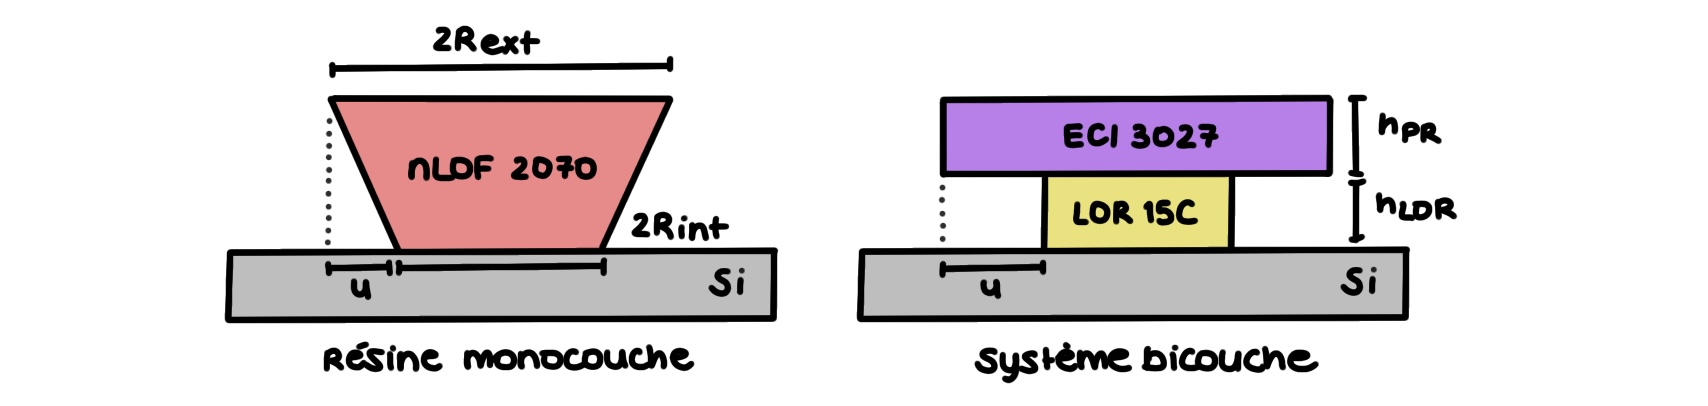
\includegraphics[width=\linewidth]{rapport-micro332/photos/s3_figure_prrocessus.jpg}
  \caption{Principe des mesures géométriques : à gauche, résine négative monocouche (diamètre $2R_{\text{ext}}$ au sommet, plan focal $p$, et $2R_{\text{int}}$ à la base, plan focal $p'$) ; à droite, coupe du système bicouche en surplomb.}
  \label{fig:s3-schema}
\end{figure}

\paragraph{Méthode de mesure.}
Les dimensions sont relevées directement avec les outils de mesure des logiciels d'acquisition (lignes parallèles, cercles ajustés ou mesure point-à-point au microscope ; cotes verticales au MEB).

\subsection{Résultats}

\paragraph{Mesures optiques des profils d'undercut.}
Les clichés métrologiques des échantillons S1 à S4 sont regroupés sur la figure~\ref{fig:s3-optique} et leurs dimensions sont synthétisées dans le tableau~\ref{tab:s3-optique}.

\begin{figure}[H]
  \centering
  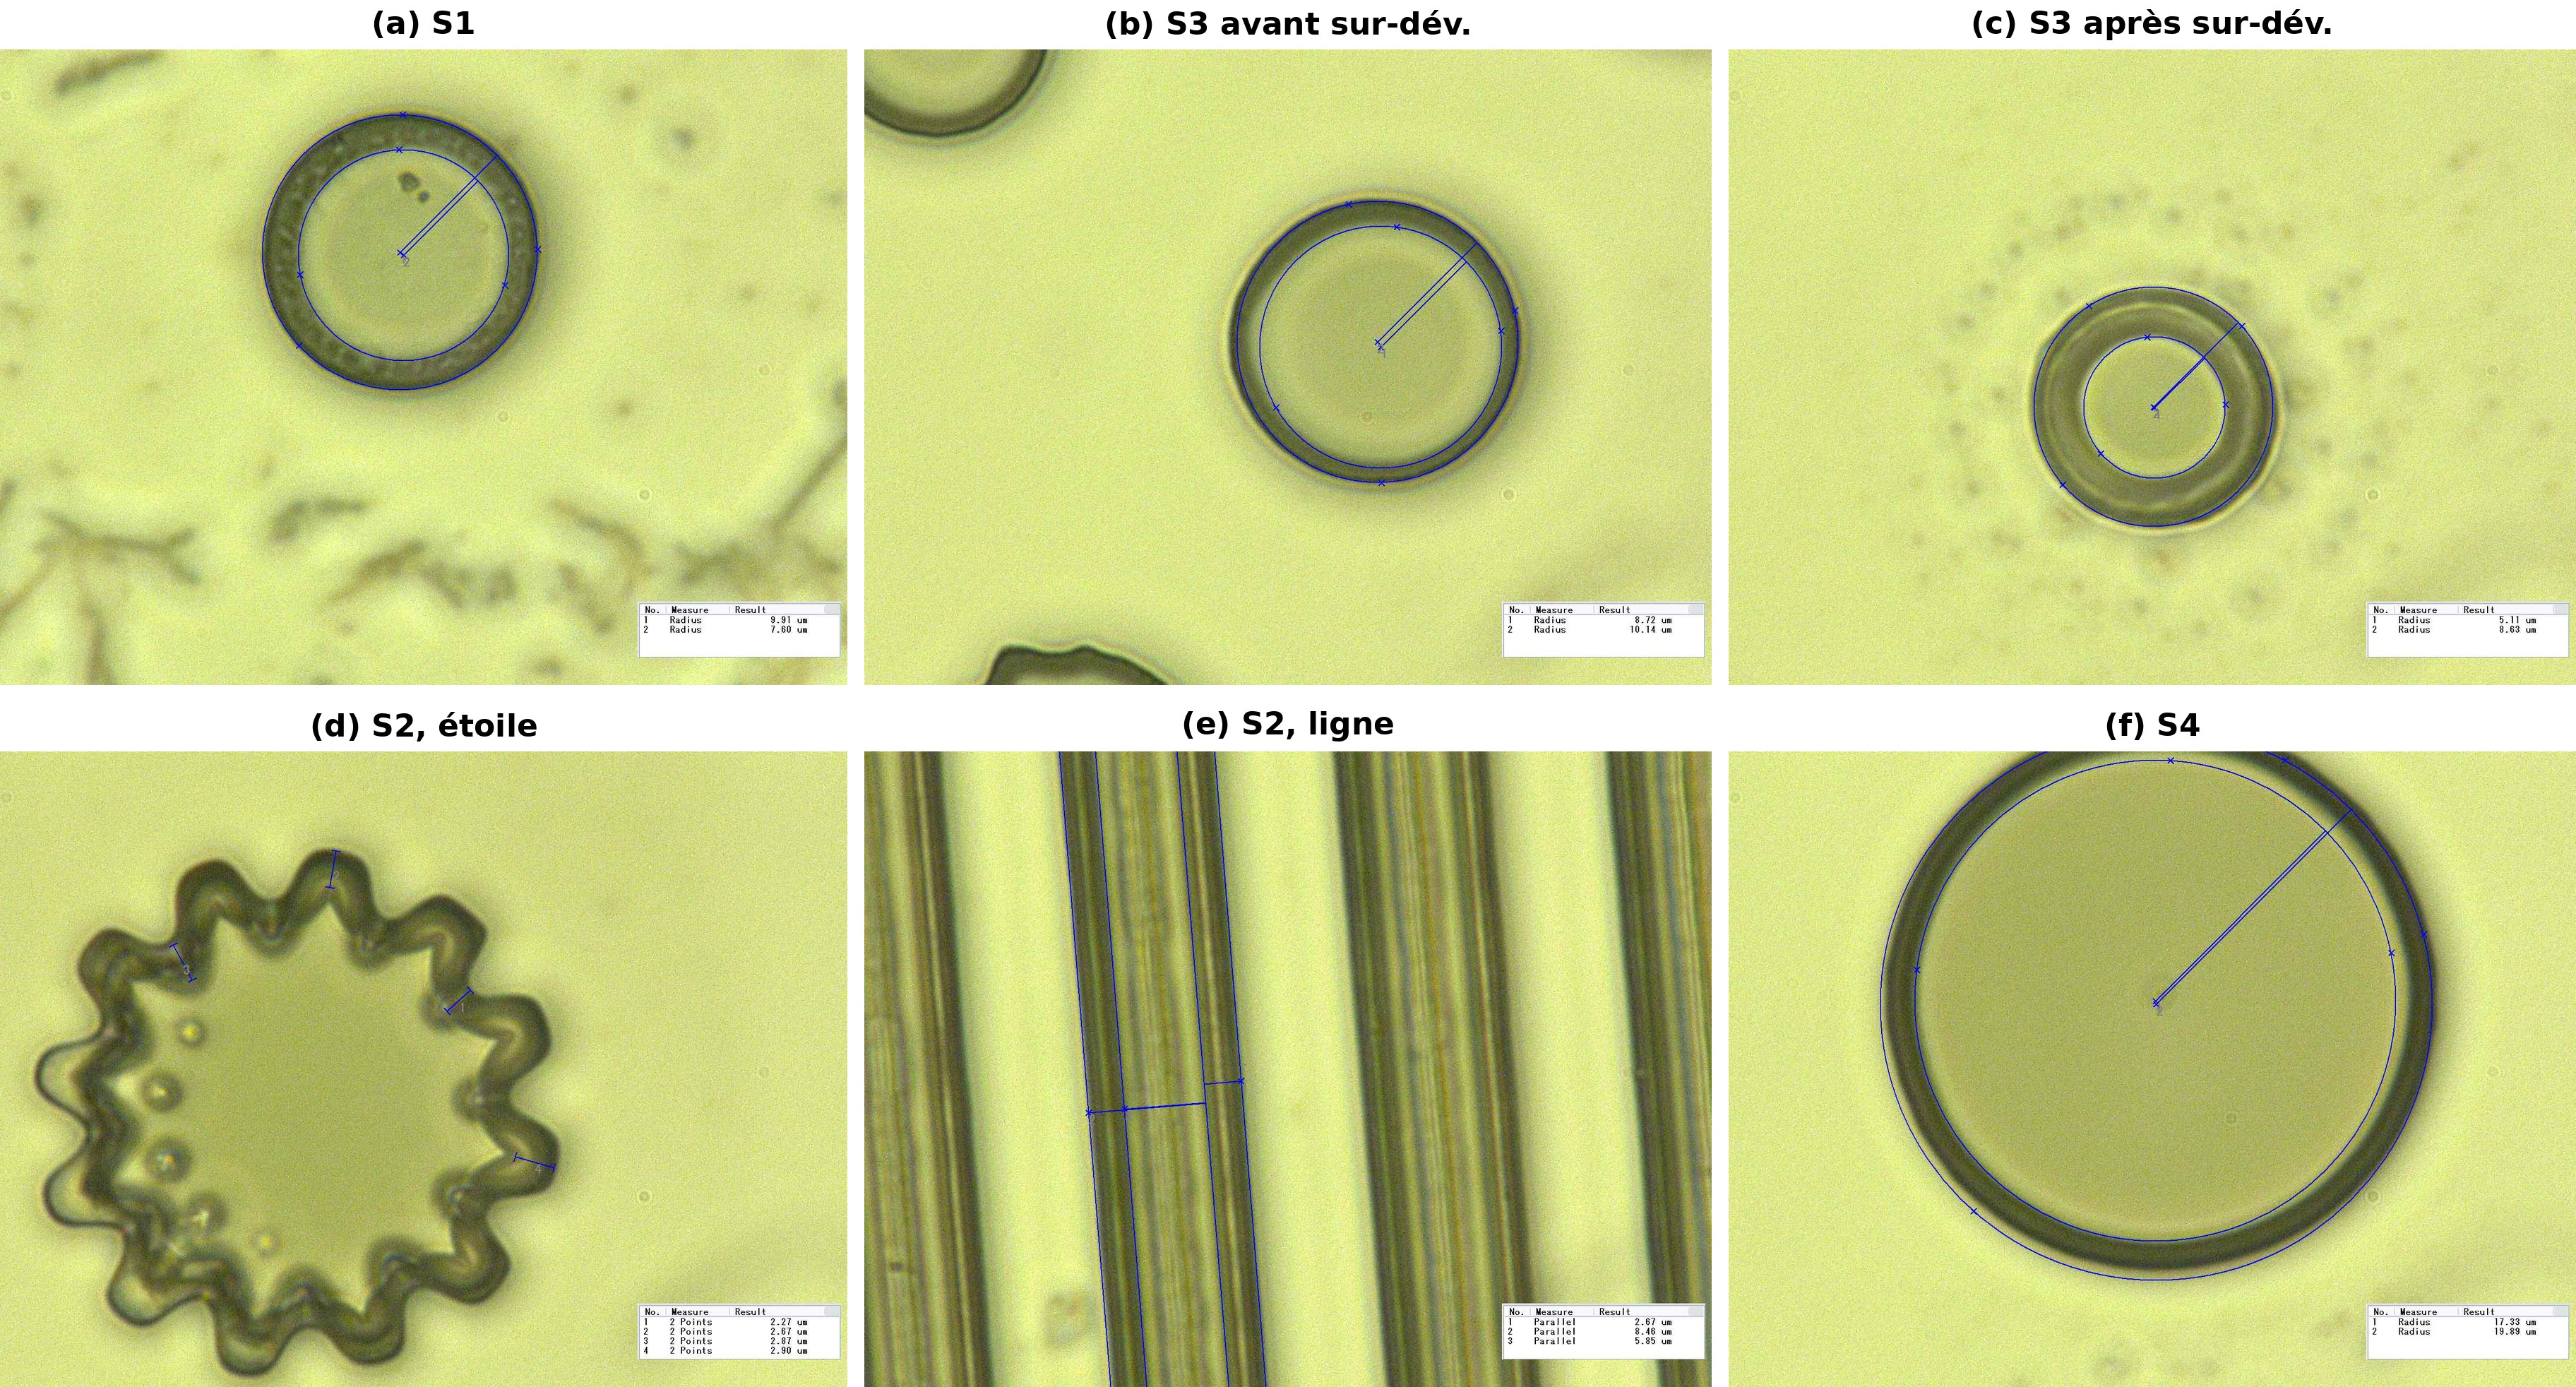
\includegraphics[width=\linewidth]{photos/fig3_2_optique_brut.jpg}
  \caption{Captures brutes au microscope optique avec les mesures du logiciel (encadré en bas à droite) : (a) S1 (nLOF, \qty{58}{\second}) ; (b) S3 avant sur-développement (\qty{62}{\second}) ; (c) S3 après +\qty{15}{\second} de sur-développement ; (d--e) S2 (bicouche, \emph{prebake} \qty{3}{\minute}) ; (f) S4 (bicouche, \emph{prebake} \qty{5}{\minute}).}
  \label{fig:s3-optique}
\end{figure}

\begin{table}[H]
  \centering\footnotesize
  \setlength{\tabcolsep}{3.5pt}
  \caption{Synthèse des mesures optiques de l'\emph{undercut} latéral $u$ et calcul de l'angle de pente $\alpha = \arctan(u/h)$.}
  \label{tab:s3-optique}
  \begin{tabularx}{\linewidth}{@{}X c c c c c c@{}}
    \toprule
    \textbf{Échantillon \& Motif} & \textbf{top} (\unit{\micro\metre}) & \textbf{bottom} (\unit{\micro\metre}) & $\mathbf{\Delta}$ (\unit{\micro\metre}) & $\mathbf{u}$ (\unit{\micro\metre}) & $\mathbf{h}$ (\unit{\micro\metre}) & $\mathbf{\alpha}$ (\unit{\degree}) \\
    \midrule
    \textbf{S1} (nLOF, \qty{58}{\second}) --- Cercle & 19,82 & 15,20 & 4,62 & \textbf{2,31}\textsuperscript{a} & 6,75 & \textbf{18,9} \\
    \textbf{S3} avant sur-dév. (\qty{62}{\second}) --- Cercle & 20,28 & 17,44 & 2,84 & \textbf{1,42} & 6,05 & \textbf{13,2} \\
    \textbf{S3} après +\qty{15}{\second} --- Cercle / Ligne & 17,26 & 10,22 & 7,04 & \textbf{3,52}\textsuperscript{b} & 6,05 & \textbf{30,2} \\
    \textbf{S2} (Bicouche, \qty{3}{\minute}) --- Étoile / Ligne & --- & --- & --- & \textbf{2,68}\textsuperscript{c} & 3,07 & --- \\
    \textbf{S4} (Bicouche, \qty{5}{\minute}) --- Cercle / Ligne & 39,78 & 34,66 & 5,12 & \textbf{2,56}\textsuperscript{d} & 2,91 & --- \\
    \bottomrule
  \end{tabularx}
  \vspace{2pt}
  \raggedright\scriptsize
  \textsuperscript{a}\,Mesure parallèle sur rectangle : \qty{1,76}{\micro\metre}.
  \textsuperscript{b}\,Mesure sur ligne : \qty{3,04}{\micro\metre}.
  \textsuperscript{c}\,Moyenne de 4 mesures directes sur l'étoile (\qtyrange{2,27}{2,90}{\micro\metre}) ; sur ligne, les deux bandes mesurent \qty{2,67}{\micro\metre} et \qty{2,61}{\micro\metre} (8,46 $-$ 5,85).
  \textsuperscript{d}\,Mesure sur ligne : \qty{2,38}{\micro\metre}. Pour S2 et S4, $h$ correspond à l'épaisseur du LOR 15C ; le profil est une marche (ECI en surplomb au-dessus du LOR) et non un flanc incliné, $\alpha$ n'est donc pas défini.
\end{table}

\paragraph{Observations en coupe transversale au MEB.}
Les clichés MEB acquis en vue inclinée (figure~\ref{fig:s3-meb}) illustrent la différence entre le flanc rétrograde continu de la résine négative AZ nLOF 2070 et le surplomb franc du système bicouche ECI 3027 / LOR 15C. Les cotes verticales mesurées sont résumées dans le tableau~\ref{tab:s3-meb}.

\begin{figure}[H]
  \centering
  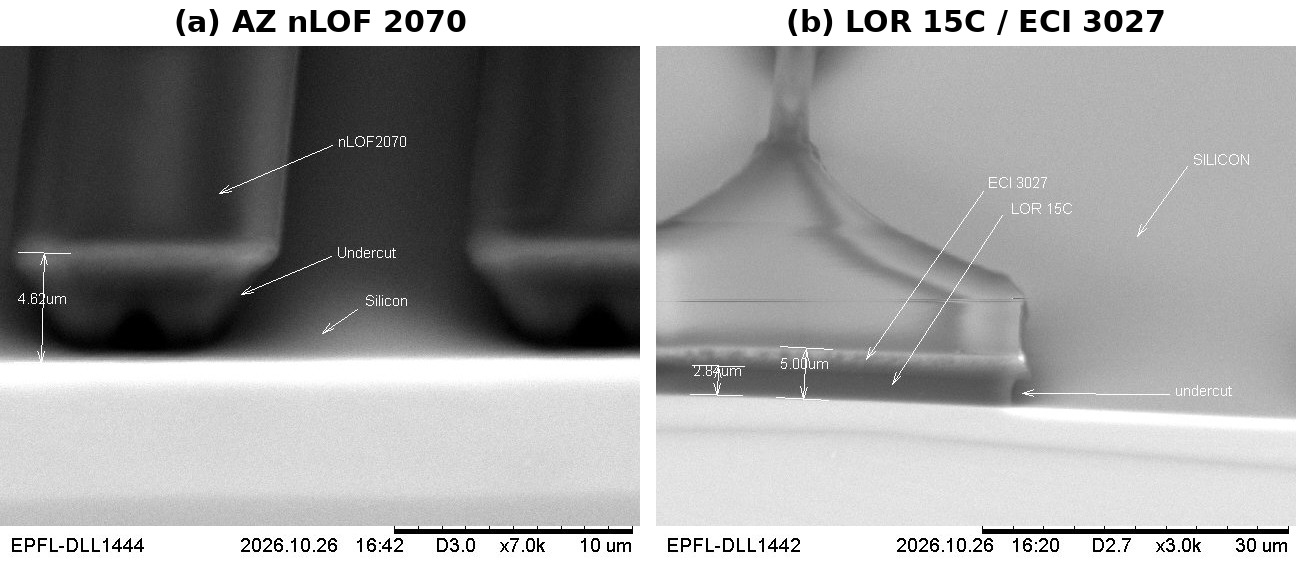
\includegraphics[width=\linewidth]{photos/fig3_3_meb_brut.jpg}
  \caption{Clichés MEB bruts (électrons rétrodiffusés, \qty{15}{\kilo\volt}, vue inclinée), avec les annotations et cotes faites pendant la séance : (a) flanc rétrograde continu de l'AZ nLOF 2070 ($\times 7{,}0\text{k}$, $h_{\text{app}} = \qty{4,62}{\micro\metre}$) ; (b) surplomb franc du bicouche ECI 3027 / LOR 15C ($\times 3{,}0\text{k}$, $h_{\text{LOR}} = \qty{2,84}{\micro\metre}$, $h_{\text{tot}} = \qty{5,00}{\micro\metre}$).}
  \label{fig:s3-meb}
\end{figure}

\begin{table}[H]
  \centering\footnotesize
  \caption{Dimensions verticales mesurées sur les clichés MEB en coupe et comparaison avec le Sujet~2.}
  \label{tab:s3-meb}
  \begin{tabularx}{\linewidth}{@{}X c c c@{}}
    \toprule
    \textbf{Grandeur mesurée en coupe MEB} & \textbf{Unité} & \textbf{Monocouche AZ nLOF 2070} & \textbf{Bicouche LOR 15C / ECI 3027} \\
    \midrule
    Hauteur couche inférieure ($h_{\text{LOR}}$) & \unit{\micro\metre} & --- & \textbf{2,84} \emph{(vs 2,91--3,07 Filmetrics)} \\
    Hauteur résine supérieure ($h_{\text{PR}}$) & \unit{\micro\metre} & \textbf{4,62} \emph{(projetée sous inclinaison)} & \textbf{2,16} \emph{(5,00 $-$ 2,84)} \\
    Hauteur totale ($h_{\text{tot}}$) & \unit{\micro\metre} & \textbf{4,62} \emph{(réelle 6,05--6,75)} & \textbf{5,00} \emph{(LOR + ECI)} \\
    Géométrie de l'\emph{undercut} & --- & Flanc incliné rétrograde continu & Surplomb horizontal franc (\emph{overhang}) \\
    \bottomrule
  \end{tabularx}
\end{table}

\paragraph{Mesure optique des largeurs de pistes TLM.}
Les largeurs optiques $W_{\text{opt}}$ des pistes d'aluminium mesurées sous les structures TLM (échantillon \emph{lift-off} du Sujet~2 et échantillon gravé du Sujet~4) sont rassemblées dans le tableau~\ref{tab:s3-tlm}. Aucune capture photographique n'a été enregistrée au microscope pour ces motifs lors de la séance.

\begin{table}[H]
  \centering\footnotesize
  \setlength{\tabcolsep}{4pt}
  \caption{Comparaison des largeurs optiques $W_{\text{opt}}$ des pistes d'aluminium TLM par rapport aux cotes nominales du masque $W_{\text{mask}}$ (Données empruntées au Groupe n°6 car nous n'avions pas les photos des pistes).}
  \label{tab:s3-tlm}
  \begin{tabularx}{\linewidth}{@{}X c c c c c c@{}}
    \toprule
    \textbf{Largeur nominale masque $W_{\text{mask}}$ (\unit{\micro\metre})} & \textbf{80} & \textbf{60} & \textbf{40} & \textbf{30} & \textbf{20} & \textbf{10} \\
    \midrule
    \textbf{Lift-Off (Sujet~2)} : $W_{\text{opt}}$ (\unit{\micro\metre}) & 82,6 & 62,8 & 42,1 & 32,0 & 21,4 & 10,9 \\
    \quad Écart $\Delta W = W_{\text{opt}} - W_{\text{mask}}$ (\unit{\micro\metre}) & $+2{,}6$ & $+2{,}8$ & $+2{,}1$ & $+2{,}0$ & $+1{,}4$ & $+0{,}9$ \\
    \quad Erreur relative (\%) & $+3{,}3$\,\% & $+4{,}7$\,\% & $+5{,}3$\,\% & $+6{,}7$\,\% & $+7{,}0$\,\% & $+9{,}0$\,\% \\
    \addlinespace[3pt]
    \textbf{Gravure (Sujet~4)} : $W_{\text{opt}}$ (\unit{\micro\metre}) & 80,0 & 59,5 & 36,4 & 26,8 & 16,9 & 7,4 \\
    \quad Écart $\Delta W = W_{\text{opt}} - W_{\text{mask}}$ (\unit{\micro\metre}) & $0{,}0$ & $-0{,}5$ & $-3{,}6$ & $-3{,}2$ & $-3{,}1$ & $-2{,}6$ \\
    \quad Erreur relative (\%) & $0{,}0$\,\% & $-0{,}8$\,\% & $-9{,}0$\,\% & $-10{,}7$\,\% & $-15{,}5$\,\% & $-26{,}0$\,\% \\
    \bottomrule
  \end{tabularx}
\end{table}

\FloatBarrier
\subsection{Analyse}

\paragraph{Analyse des données et des observations.}
\begin{enumerate}
  \item \textbf{Profils d'undercut en optique (tableau~\ref{tab:s3-optique}) :} Sur S1 (nLOF 2070, \qty{58}{\second}, $h = \qty{6,75}{\micro\metre}$), on mesure $u = \qty{2,31}{\micro\metre}$ sur cercle ($\alpha = \qty{18,9}{\degree}$) et \qty{1,76}{\micro\metre} sur rectangle. Sur S3 (\qty{62}{\second}, $h = \qty{6,05}{\micro\metre}$), la dose plus élevée limite le retrait initial à $u = \qty{1,42}{\micro\metre}$ ($\alpha = \qty{13,2}{\degree}$), mais le sur-développement de \qty{15}{\second} creuse la base jusqu'à $u = \qty{3,52}{\micro\metre}$ ($\alpha = \qty{30,2}{\degree}$). Pour le bicouche, S2 (\emph{prebake} \qty{3}{\minute}) atteint $u = \qty{2,68}{\micro\metre}$ en moyenne contre $u = \qty{2,56}{\micro\metre}$ pour S4 (\emph{prebake} \qty{5}{\minute}), avec la même insolation et le même développement. L'écart va dans le sens attendu, un LOR 15C moins recuit se gravant plus vite latéralement \cite{lor}, mais il reste du même ordre que la dispersion sur l'étoile (\qtyrange{2,27}{2,90}{\micro\metre}) et ne repose que sur deux échantillons.
  \item \textbf{Confrontation MEB et Filmetrics (tableau~\ref{tab:s3-meb}) :} Sur le système bicouche, la coupe MEB distingue nettement le LOR 15C ($h_{\text{LOR}} = \qty{2,84}{\micro\metre}$, en accord avec les \qtyrange{2,91}{3,07}{\micro\metre} Filmetrics) et l'ECI 3027 ($h_{\text{PR}} = \qty{2,16}{\micro\metre}$, total \qty{5,00}{\micro\metre}), avec une cavité d'\emph{undercut} franche à la base. Sur l'AZ nLOF 2070, le flanc est incliné de façon continue et la hauteur apparente (\qty{4,62}{\micro\metre}) est inférieure à l'épaisseur réelle (\qtyrange{6,05}{6,75}{\micro\metre}) du fait de l'inclinaison du porte-échantillon ($h_{\text{app}} = h_{\text{réel}}\sin\theta$, soit $\theta \approx$ \qtyrange{43}{50}{\degree} ; cet angle n'est pas enregistré par le MEB et nous le déduisons ici des épaisseurs Filmetrics). Les hauteurs du bicouche ne sont pas corrigées : leur accord avec le Filmetrics suppose que sa tranche a été vue presque de face.
  \item \textbf{Fidélité dimensionnelle des pistes TLM (tableau~\ref{tab:s3-tlm}) :} Les pistes obtenues par \emph{lift-off} sont systématiquement légèrement plus larges que le masque ($\Delta W$ compris entre $+0{,}9$ et \qty{+2,8}{\micro\metre}), tout en restant proches de la cote nominale même à \qty{10}{\micro\metre} (\qty{10,9}{\micro\metre}, soit $+9{,}0$\,\%). À l'inverse, la gravure humide réduit la largeur des pistes de \qtyrange{2,6}{3,6}{\micro\metre} pour $W_{\text{mask}} \le \qty{40}{\micro\metre}$ (soit environ \qtyrange{1,3}{1,8}{\micro\metre} de sous-gravure par côté), portant la perte relative à $-26{,}0$\,\% sur la piste de \qty{10}{\micro\metre} (\qty{7,4}{\micro\metre}). Les pistes très larges (\qty{80}{\micro\metre} et \qty{60}{\micro\metre}) présentent un écart quasi nul ($0{,}0$ à \qty{-0,5}{\micro\metre}). Une gravure isotrope devrait pourtant enlever la même largeur sur chaque bord, quelle que soit la piste : cet écart nul relève plutôt de la mesure (données du groupe~6, sans image pour la vérifier). Au sujet~6, le TLM du groupe~10 donne d'ailleurs une perte constante de \qty{2,5}{\micro\metre}, y compris à \qty{80}{\micro\metre}.
\end{enumerate}

\paragraph{Interprétation physique et discussion.}
Dans l'AZ nLOF 2070, la pente rétrograde ($\alpha = \qty{18,9}{\degree}$ à \qty{30,2}{\degree}) crée l'ombrage nécessaire lors de l'évaporation directionnelle, mais le sur-développement réduit l'assise au sol (sur S3, le diamètre à la base passe de \qty{17,44}{\micro\metre} à \qty{10,22}{\micro\metre}), fragilisant les motifs fins. Le système bicouche maintient une base large en LOR 15C sous un surplomb franc d'environ \qty{2,6}{\micro\metre} en ECI 3027, ce qui doit permettre une rupture nette du métal (S2 et S4 n'ont pas été métallisés). Sur les pistes TLM, le léger élargissement observé en \emph{lift-off} pourrait venir d'une ouverture au sommet de la résine un peu plus large que le masque, puisque c'est le bord du surplomb qui fixe la largeur du métal en évaporation directionnelle ; le TLM du sujet~6 (groupe~10) trouve au contraire des lignes à moins de \qty{1}{\micro\metre} de la cote du masque. Le rétrécissement en gravure résulte du caractère isotrope de l'attaque chimique humide sous le masque \cite{intro}. Enfin, la mesure optique se fait à travers la résine, en changeant de plan focal entre le sommet et la base, et le placement des bords reste approximatif : sur l'étoile de S2, nos quatre mesures vont de 2,27 à \qty{2,90}{\micro\metre}. Le MEB montre directement le profil en coupe, au prix d'une préparation destructive (clivage) et d'un risque de charge électrostatique des polymères ; nous n'y avons toutefois mesuré que des hauteurs, pas la largeur du surplomb.

\subsection{Conclusion}
La microscopie optique et le MEB ont permis de quantifier les profils d'\emph{undercut} du Sujet~2. Le sur-développement de \qty{15}{\second} sur S3 (\qty{62}{\second}) a porté son retrait latéral de \qty{1,42}{\micro\metre} ($\alpha = \qty{13,2}{\degree}$) à \qty{3,52}{\micro\metre} ($\alpha = \qty{30,2}{\degree}$), tandis que le système bicouche produit un surplomb régulier de \qtyrange{2,56}{2,68}{\micro\metre}, légèrement plus large pour le \emph{prebake} le plus court (\qty{3}{\minute} contre \qty{5}{\minute}), et dont la présence est confirmée en coupe MEB ($h_{\text{LOR}} = \qty{2,84}{\micro\metre}$). Sur les pistes TLM, le \emph{lift-off} assure une meilleure fidélité sur les motifs fins ($+9{,}0$\,\% à \qty{10}{\micro\metre}) que la gravure humide, dont la sous-gravure isotrope induit jusqu'à $-26{,}0$\,\% de perte de largeur.

\clearpage
% ==================================================================
%  Sujet 4 : Gravure de l'aluminium et alignement de masque
%  Seance du 9 novembre 2026, DLL-MED
% ==================================================================
\section{Gravure de l'aluminium et alignement de masque}

\subsection{Objectif}

\noindent Ce sujet vise à mettre en pratique deux étapes essentielles de la photolithographie : la gravure sélective d’une couche d’aluminium et l’alignement d’un photomasque sur des motifs préexistants \cite{intro,prot4}.

\noindent La première partie consiste à transférer des motifs sur une couche d’aluminium par photolithographie, suivie d’une gravure chimique humide. L’objectif est de déterminer le temps nécessaire à la gravure pour les deux types de chip utilisés : du verre et du silicium, en plus d’observer les motifs obtenus au microscope optique.

\noindent La seconde partie consiste à aligner précisément un photomasque avec des structures déjà présentes sur un wafer, afin de réaliser une nouvelle exposition UV et d'évaluer la qualité de l'alignement.

\subsection{Matériels}
Le matériel est listé au tableau~\ref{tab:s4-materiel}.

\begin{table}[htbp]
  \centering\small
  \caption{Matériel utilisé pendant la séance.}
  \label{tab:s4-materiel}
  \begin{tabularx}{\linewidth}{@{}lX@{}}
    \toprule
    \textbf{Catégorie} & \textbf{Utilisé pendant la séance} \\
    \midrule
    Équipements & chips en verre et silicium recouverts d'aluminium, wafer de silicium avec motifs, plaque chauffante, spin coater, aligneur de masque UV, photomasques, microscope optique, hotte chimique, béchers, pistolet à azote \\
    Produits chimiques & résine positive AZ1512 \cite{tdsaz1500}, révélateur AZ 726 MIF, solution de gravure de l'aluminium A (mélange d'acide acétique, nitrique et phosphorique), acétone, alcool isopropylique, eau déionisée (DI) \\
    \bottomrule
  \end{tabularx}
\end{table}


\subsection{Méthodes}

\subsubsection{Étapes expérimentales}

\noindent\textbf{A. Gravure de l'aluminium}

\begin{figure}[htbp]
    \centering
    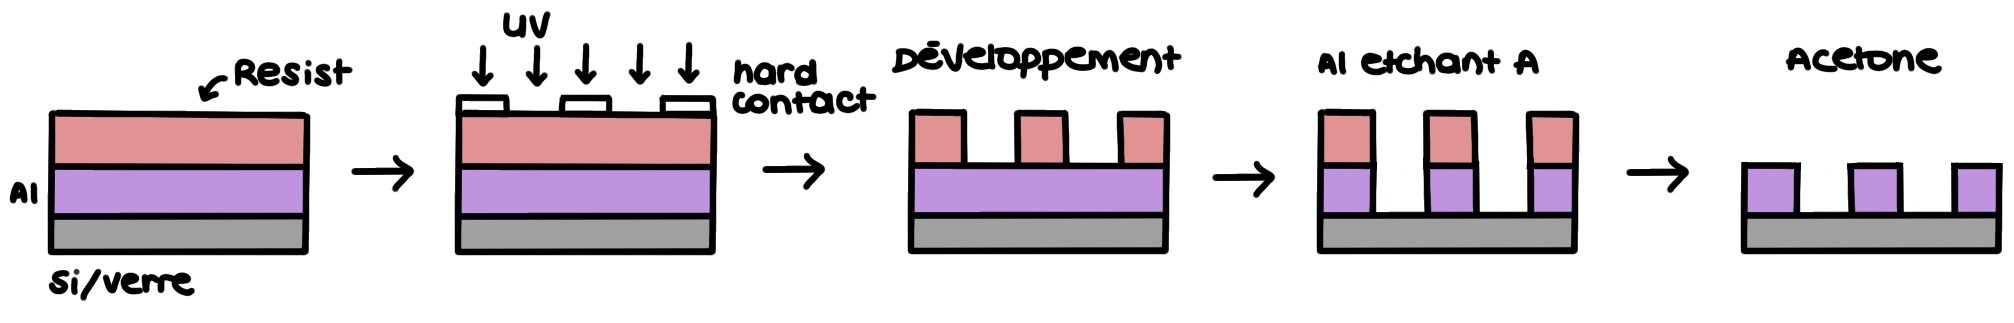
\includegraphics[width=\textwidth]{rapport-micro332/photos/s4_gravure_alu.jpg}
    \caption{Étapes de la gravure de l'aluminium}
    \label{fig:s4_gravure_aluminium}
\end{figure}

Pour chaque chip, en verre et en silicium, on suit les étapes de la figure~\ref{fig:s4_gravure_aluminium} :

\begin{enumerate}

    \item \textbf{Préparation du chip :}
    Le chip est déshydraté sur une plaque chauffante à \qty{150}{\celsius} pendant \qty{2}{\minute} (cette étape a été réalisée avant le début du TP). Une couche de résine positive AZ1512 est ensuite déposée par centrifugation, en deux étapes successives : \qty{700}{\tour\per\minute} pendant \qty{7}{\second}, puis \qty{4000}{\tour\per\minute} pendant \qty{60}{\second}. Un soft bake est réalisé à \qty{100}{\celsius} pendant \qty{60}{\second}.

    \item \textbf{Photolithographie :}
    Le chip est exposé aux UV à travers un photomasque pendant \qty{10}{\second}, en hard contact. La résine est ensuite développée dans une solution AZ 726 MIF pendant \qty{45}{\second}, sous agitation douce. Après un rinçage à l'eau DI pendant \qty{1}{\minute} et un séchage à l'azote, une cuisson supplémentaire (post-bake) est effectuée à \qty{100}{\celsius} pendant \qty{90}{\second} afin de durcir la résine restante.

    \item \textbf{Inspection initiale :}
    Les motifs obtenus sont observés au microscope optique et une image de référence est enregistrée.

    \item \textbf{Gravure chimique :}
    Le chip est immergé dans une solution Aluminum Etchant A, maintenue à \qty{40}{\celsius} et constituée d'acides phosphorique, nitrique et acétique ainsi que d'eau DI, dans un rapport volumique de 16:1:1:2. Le temps nécessaire à l'élimination complète de l'aluminium non protégé par la résine est mesuré pour les deux chips. Le chip est ensuite rincé successivement dans deux bains d'eau DI pendant \qty{3}{\minute} chacun, puis séché.

    \item \textbf{Inspection finale :}
    Les motifs gravés sont observés au microscope optique. La résine restante est ensuite retirée à l'acétone, suivie d'un rinçage à l'IPA et à l'eau DI.

\end{enumerate}

\noindent\textbf{B. Alignement du photomasque}

\begin{figure}[htbp]
    \centering
    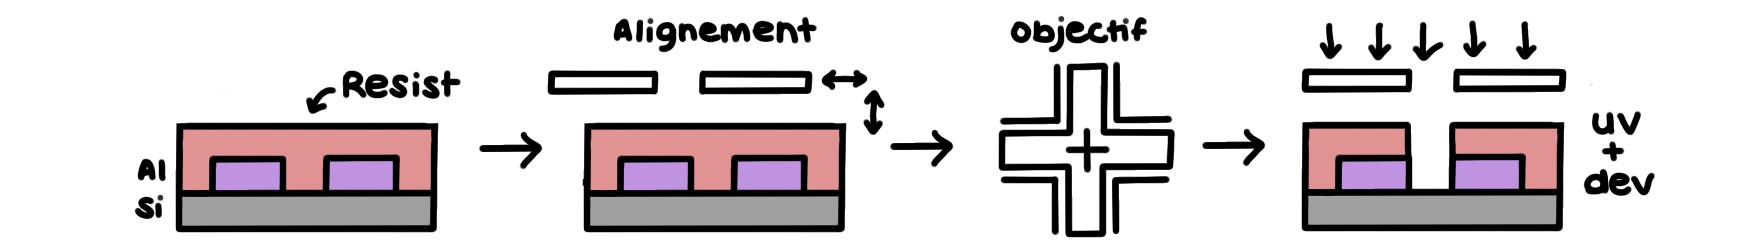
\includegraphics[width=\textwidth]{rapport-micro332/photos/s4_align_mask.jpg}
    \caption{Étapes de l'alignement de masque}
    \label{fig:s4_align_mask}
\end{figure}

De façon à positionner précisément les motifs d'un photomasque par rapport à des structures déjà présentes sur le wafer, on suit les étapes de la figure~\ref{fig:s4_align_mask} :

\begin{enumerate}

    \item \textbf{Préparation du wafer :}
    Le wafer est déshydraté à \qty{150}{\celsius} pendant \qty{5}{\minute} (cette étape a été réalisée avant le début du TP). La résine AZ1512 est déposée à \qty{700}{\tour\per\minute} pendant \qty{7}{\second}, puis à \qty{4000}{\tour\per\minute} pendant \qty{60}{\second}. Une précuisson à \qty{100}{\celsius} pendant \qty{60}{\second} est ensuite effectuée.

    \item \textbf{Mise en place :}
    Le wafer est placé au centre du support de l'aligneur et maintenu par aspiration. Le photomasque est fixé dans le support supérieur, avec sa face chromée orientée vers le wafer. Le wafer est progressivement rapproché du masque jusqu'à un léger contact permettant de rendre leurs surfaces parallèles. Le mécanisme de parallélisation est ensuite verrouillé.

    \item \textbf{Alignement :}
    Le wafer est abaissé afin d'établir un écart de \qtyrange{20}{50}{\micro\metre} avec le masque. Un premier alignement approximatif est réalisé visuellement, puis les positions X, Y et l'orientation angulaire $\theta$ sont ajustées à l'aide des micromètres et des microscopes numériques, jusqu'à la superposition des marques d'alignement. Le wafer est ensuite remis en contact avec le masque et l'alignement est vérifié.

    \item \textbf{Exposition et développement :}
    Une exposition UV de \qty{10}{\second} est réalisée en mode contact dur. Le wafer est ensuite développé dans la solution AZ 726 MIF pendant \qty{30}{\second}, sous agitation douce, puis rincé à l'eau DI et séché à l'azote.

    \item \textbf{Inspection :}
    Les motifs obtenus sont observés au microscope optique afin d'examiner leur positionnement par rapport aux structures préexistantes.

\end{enumerate}

\subsubsection{Méthodes de mesure}

\noindent\textbf{A. Gravure de l'aluminium}

Le temps de gravure est déterminé en chronométrant la durée d'immersion nécessaire à l'élimination complète de l'aluminium dans les zones non protégées par la résine. La gravure est ensuite contrôlée par observation au microscope optique.

Des images d'un même motif sont acquises après le développement et après la gravure pour comparer l'aspect des structures.
\\


\noindent\textbf{B. Alignement du photomasque}

L'alignement est réalisé par observation simultanée des marques de référence du wafer et du photomasque à l'aide des microscopes numériques USB intégrés à l'aligneur. Les décalages en X, Y et $\theta$ sont corrigés progressivement jusqu'à obtenir une superposition satisfaisante des marques.

Après exposition et développement, la qualité de l'alignement est évaluée par inspection au microscope optique, en comparant la position des nouveaux motifs avec celle des structures préexistantes.


\subsection{Résultats}

\noindent\textbf{A. Gravure de l'aluminium}

Le premier binôme a réalisé la gravure sur silicium et le deuxième sur verre. La figure~\ref{fig:tp4_gravure} compare les mêmes types de motifs et structures sur les deux substrats après développement et après gravure.

\begin{figure}[htbp]
    \centering
    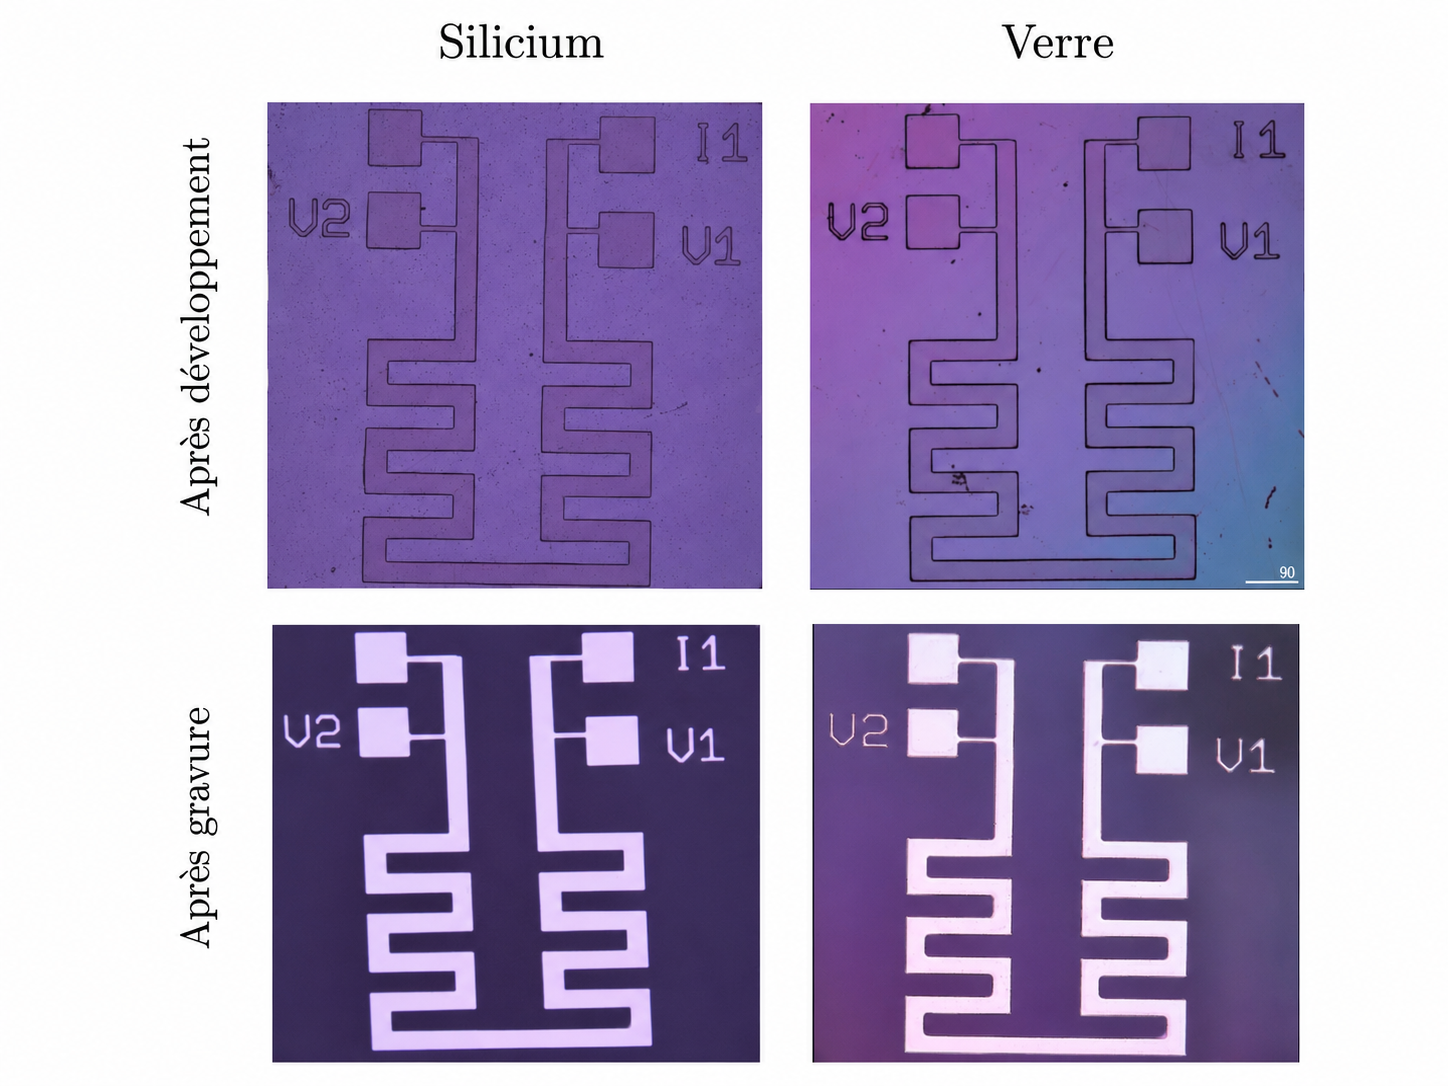
\includegraphics[width=0.72\textwidth]{rapport-micro332/photos/s4_comparaison_gravure.png}
    \caption{Comparaison des motifs observés sur silicium et sur verre.}
    \label{fig:tp4_gravure}
\end{figure}

Sur les deux substrats, les motifs sont bien visibles et les lignes semblent continues. On observe toutefois quelques petits défauts sur les bords des motifs, particulièrement sur les images du verre.

\begin{table}[htbp]
    \centering\small
    \caption{Temps de gravure de l'aluminium mesurés au chronomètre.}
    \label{tab:tp4_gravure}
    \begin{tabular}{@{}lc@{}}
        \toprule
        Substrat & Temps de gravure \\
        \midrule
        Silicium & \qty{4}{\minute}~\qty{13}{\second} \\
        Verre & \qty{4}{\minute}~\qty{37}{\second} \\
        \bottomrule
    \end{tabular}
\end{table}

\noindent\textbf{B. Alignement du photomasque}

L'alignement a été réalisé par chaque binôme sur le même type de wafer en silicium. La figure~\ref{fig:tp4_alignement} présente le repère « 2 » et une croix centrale, photographiés pour chacun des deux binômes.

\begin{figure}[htbp]
    \centering
    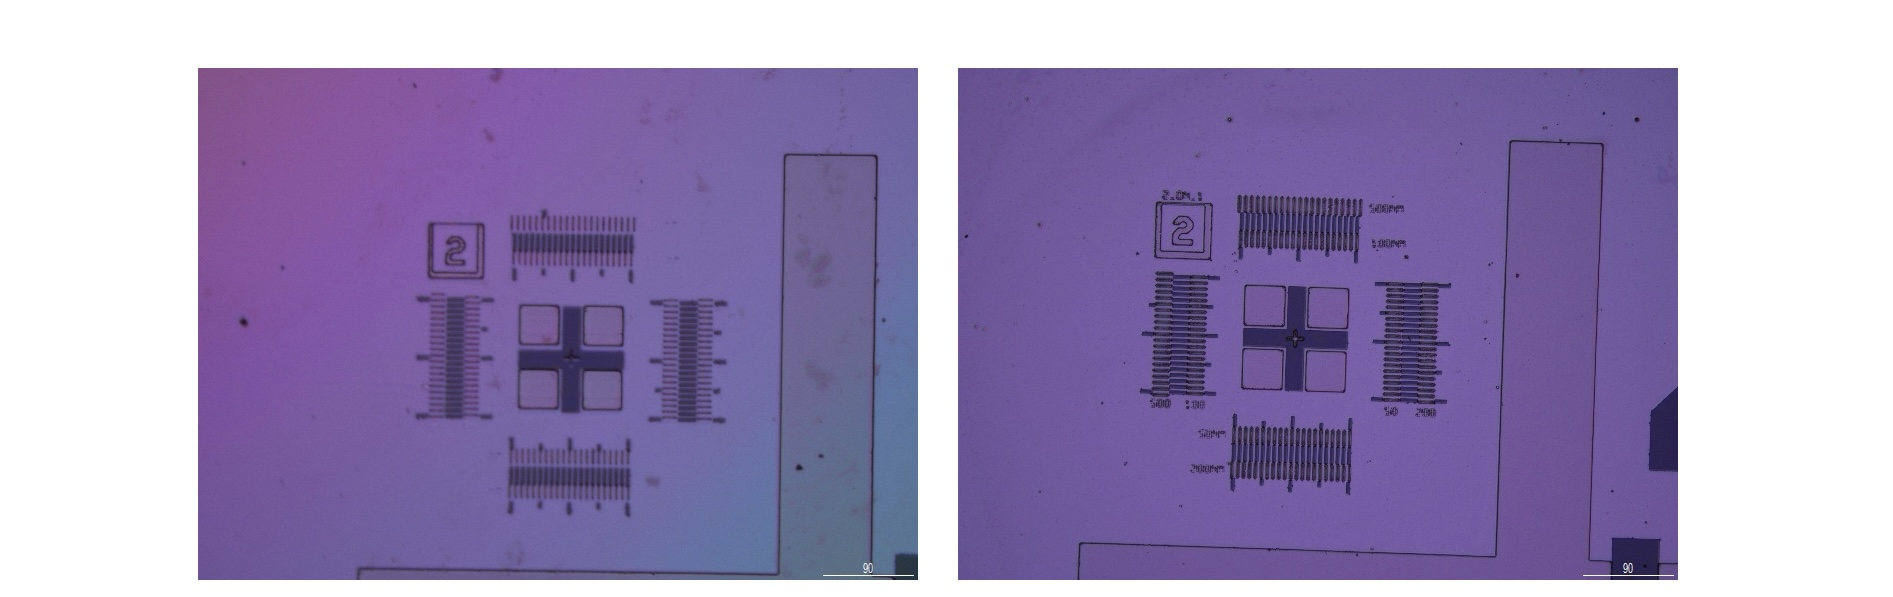
\includegraphics[width=0.72\textwidth]{rapport-micro332/photos/s4_alignement1.jpg}\\[2pt]
    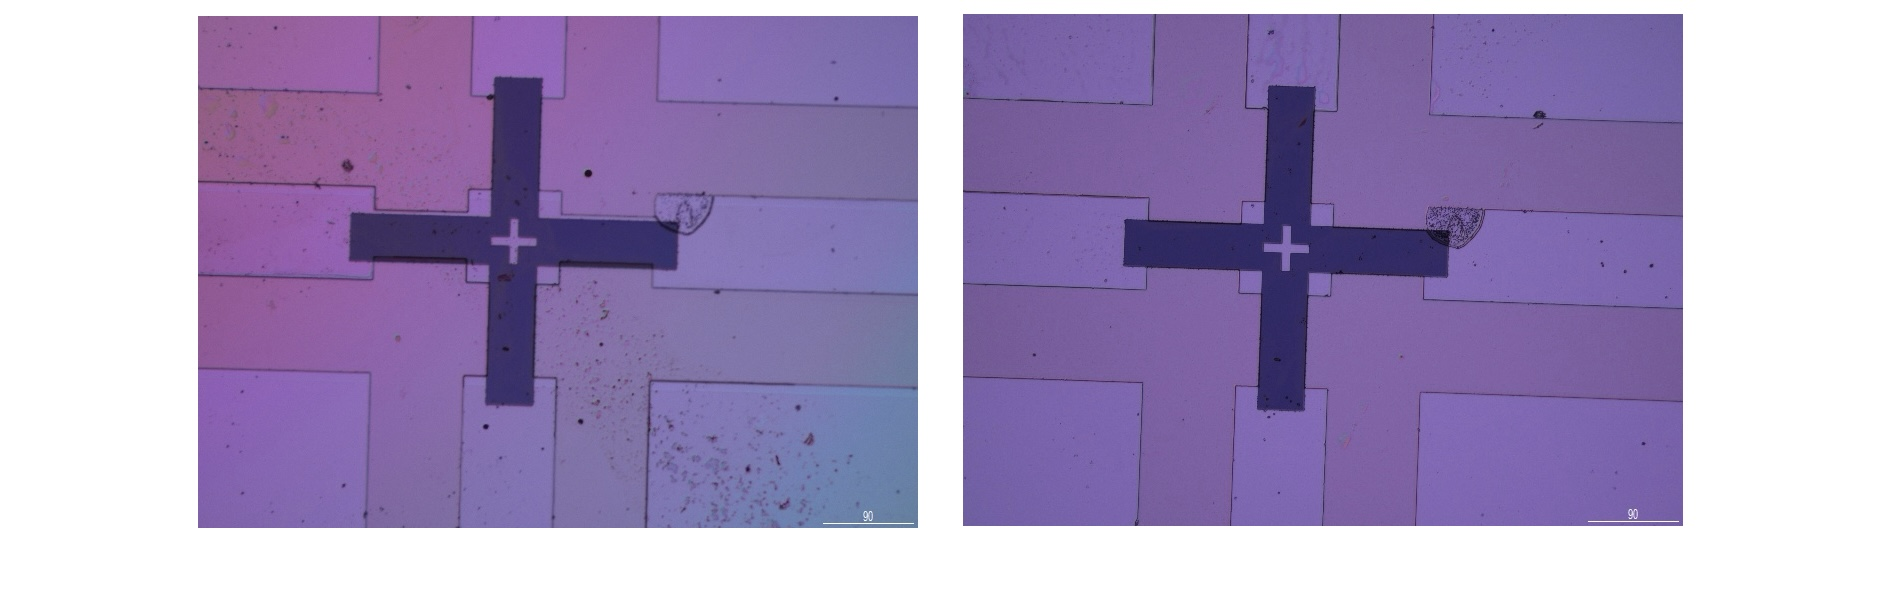
\includegraphics[width=0.72\textwidth]{rapport-micro332/photos/s4_alignement2.jpg}
    \caption{Comparaison des structures après la manipulation d'alignement pour chacun des binômes. En haut : zone de référence « 2 ». En bas : croix centrale.}
    \label{fig:tp4_alignement}
\end{figure}

Dans les deux séries, une croix sombre apparaît autour d'une croix claire, qui sert de repère pour l'alignement visuel des motifs.

\subsection{Analyse}

\noindent\textbf{A. Gravure de l'aluminium}

Les structures obtenues et les temps de gravure sont globalement similaires sur les deux substrats, ce qui indique un transfert réussi des motifs. Les petites imperfections visibles après le développement, probablement dues à des particules ou à des résidus de résine, ne sont plus observables après la gravure.

Les deux temps de gravure (tableau~\ref{tab:tp4_gravure}) diffèrent de \qty{24}{\second}, soit \qty{9}{\percent}. La solution attaque l'aluminium et pas le substrat : à épaisseur d'Al égale, on attend donc des temps proches sur verre et sur silicium. Le temps dépend en revanche surtout de l'épaisseur d'Al, de la température du bain (\qty{40}{\celsius}) et de l'agitation. L'écart restant peut venir d'une différence d'épaisseur entre les deux chips, d'un bain un peu refroidi entre les deux gravures, ou du jugement visuel de la fin de gravure par deux binômes différents, plus délicat sur le verre transparent. La vitesse de gravure de l'Al double environ tous les \qty{5}{\celsius} \cite{alumicro} : un écart de \qty{9}{\percent} correspond à moins de \qty{1}{\celsius} de différence de bain. Le départ de la gravure varie aussi : le développeur attaque déjà l'alumine native là où la résine est ouverte, et les bulles d'hydrogène rendent l'attaque inhomogène \cite{alumicro}. Le protocole demande enfin de comparer la taille d'un même motif avec et sans résine (étape 16) ; nos images ne contiennent pas de cliché du même motif après retrait de la résine, et cette comparaison n'a pas pu être faite.

Les différences visuelles au niveau des contours s'expliquent notamment par les propriétés optiques des substrats. Le silicium, opaque et réfléchissant, offre un contraste plus marqué, tandis que la transparence du verre et les réflexions aux interfaces peuvent rendre les contours moins nets sur les images.
\\

\noindent\textbf{B. Alignement du photomasque}

Les deux alignements sont globalement satisfaisants. On observe toutefois un léger décalage selon l'axe vertical pour l'un des binômes, tandis que l'autre présente une superposition plus précise des croix et de leurs repères. Aucun décalage significatif n'est visible dans ce second cas. Ce jugement reste visuel : nous n'avons pas relevé le décalage en micromètres, ce que permettraient les verniers gradués visibles autour du repère « 2 » (figure~\ref{fig:tp4_alignement}) \cite{prot4}.

\subsection{Conclusion}

Ce sujet a permis de réaliser une gravure sélective de l'aluminium sur deux substrats différents, ainsi que l'alignement d'un photomasque sur des structures préexistantes.
\\

Les résultats montrent que la gravure produit des motifs similaires sur verre et sur silicium, avec des temps de gravure de \qty{4}{\minute}~\qty{13}{\second} et \qty{4}{\minute}~\qty{37}{\second}. Les différences visuelles observées sont probablement liées en partie aux propriétés optiques des substrats.

Enfin, les deux alignements ont été réalisés avec une précision visuellement satisfaisante, malgré un léger décalage observé dans l'un des cas. Ces manipulations illustrent l'importance du contrôle des paramètres de gravure et de la précision de l'alignement en microfabrication.




\clearpage
% ==================================================================
%  Sujet 5 : Salle blanche CMi -- lithographie automatisee et
%  gravure humide de l'aluminium
%  Seance du 12 octobre 2026 (a verifier), CMi
% ==================================================================
\section[Salle blanche CMi -- lithographie et gravure de l'Al]{Salle blanche CMi -- lithographie automatisée et gravure humide de l'aluminium}

\subsection{Objectif}
Ce sujet fait découvrir la salle blanche du CMi : ses règles, ses équipements et la manipulation correcte des plaquettes \cite{prot5}. On suit une plaquette de verre couverte d'aluminium à travers une photolithographie automatisée (EVG 150, MLA 150) et une gravure humide de l'Al, puis on mesure la marche au profilomètre. On compare enfin ce travail au travail manuel des sujets 1 et 2 en DLL-MED.

\subsection{Matériels}
\begin{table}[htbp]
  \centering\small
  \caption{Matériel utilisé pendant la séance.}
  \label{tab:s5-materiel}
  \begin{tabularx}{\linewidth}{@{}lX@{}}
    \toprule
    \textbf{Catégorie} & \textbf{Utilisé pendant la séance} \\
    \midrule
    Substrats   & Plaquette de verre de \qty{100}{\milli\metre} et \qty{500}{\micro\metre}, couverte de \qty{500}{\nano\metre} d'Al et de \qty{1}{\micro\metre} d'AZ ECI 3007 ; seconde plaquette Al/verre à enduire pour le groupe suivant \\
    Produits    & Résine AZ ECI 3007, développeur de l'EVG 150, bain ANP (\ce{H3PO4} \qty{85}{\percent}, \ce{CH3COOH} \qty{100}{\percent}, \ce{HNO3} \qty{70}{\percent} dans le rapport 83 : 5,5 : 5,5 en volume), remover 1165 ou acétone et IPA, eau DI \\
    Équipements & EVG 150 (zone 6), MLA 150-1 (zone 16), banc Plade Metal (zone 2), UFT (zone 2), profilomètre Dektak (zone 15) ; fichier GDS des résistances et des images proposées par les étudiants \\
    Tenue       & Surchaussures, combinaison, bottes, masque, charlotte, lunettes de sécurité, gants \\
    \bottomrule
  \end{tabularx}
\end{table}

\subsection{Méthodes}

\paragraph{Entrée en salle blanche.}
Assis sur le banc, on enfile les surchaussures, puis la combinaison sans que les manches touchent le sol, les bottes, le masque et la charlotte, les lunettes et les gants. On vérifie la tenue avant d'entrer. Les plaquettes se manipulent uniquement avec des pinces, sans jamais toucher leur surface.

\paragraph{Procédé.}
Les étapes 1 à 3 étaient faites à l'avance ; nous avons commencé à l'étape 4 (tableau~\ref{tab:s5-procede}, figure~\ref{fig:s5-schema}). Les machines étant complexes et coûteuses, l'assistant(e) a réalisé la plupart des étapes et nous avons observé.

\begin{table}[htbp]
  \centering\small
  \caption{Process flow réalisé au CMi \cite{prot5,mlaparam}.}
  \label{tab:s5-procede}
  \begin{tabularx}{\linewidth}{@{}clp{3.3cm}X@{}}
    \toprule
    Étape & Procédé & Équipement (zone) & Paramètres \\
    \midrule
    1  & Nettoyage piranha       & UFT Piranha (Z2)   & Substrat de verre, \qty{500}{\micro\metre} \\
    2  & Métallisation           & Spider 600 (Z4)    & Al, \qty{500}{\nano\metre} \\
    3  & Enduction de résine     & EVG 150 (Z6)       & AZ ECI 3007, \qty{1}{\micro\metre}, recette C4\_D\_3007\_1ux, sans HMDS ; faite par nous sur la plaquette du groupe suivant \\
    4a & Exposition sans masque  & MLA 150-1 (Z16)    & Laser \qty{405}{\nano\metre}, puissance \qty{100}{\percent}, dose \qty{160}{\milli\joule\per\centi\metre\squared}, défocus $-1$, mode rapide, motif inversé \averifier{paramètres réellement utilisés} \\
    4b & Développement           & EVG 150 (Z6)       & Recette de développement automatique \\
    5  & Gravure humide de l'Al  & Plade Metal (Z2), bain ANP & \qty{35}{\celsius}, environ \qty{300}{\nano\metre\per\minute}, \qtyrange{5}{10}{\minute} selon le protocole ; durée réelle : \acompleter{} \\
    6  & Retrait de la résine    & UFT (Z2)           & Remover 1165, plasma \ce{O2} ou acétone et IPA \acompleter{méthode utilisée} \\
    7  & Mesure d'épaisseur      & Dektak (Z15)       & Profilomètre à stylet \\
    \bottomrule
  \end{tabularx}
\end{table}

\begin{figure}[htbp]
  \centering
  \resizebox{\linewidth}{!}{% Figure 5.1 -- procede realise au CMi (coupes schematiques, pas a l'echelle)
% Vignettes 10 x 6 unites ; verre 0 -> 1,8 ; Al 1,8 -> 2,5 ; resine 2,5 -> 3,6.
\begin{tikzpicture}[x=0.34cm, y=0.34cm, font=\scriptsize,
    contour/.style={draw=black!75, line width=0.3pt},
    note/.style={-{Stealth[length=2.5pt]}, line width=0.35pt}]

  \newcommand{\Verre}{\fill[verre, contour] (0,0) rectangle (10,1.8);}
  \newcommand{\AlPlein}{\fill[alu, contour] (0,1.8) rectangle (10,2.5);}
  \newcommand{\AlGrave}{\fill[alu, contour] (3.95,1.8) -- (6.05,1.8) -- (5.8,2.5) -- (4.2,2.5) -- cycle;}
  \newcommand{\Titre}[1]{\node[align=center, font=\footnotesize] at (5,7.2) {#1};}

  % --- ligne du haut ---------------------------------------------------
  \begin{scope}[shift={(0,0)}]
    \Titre{1. Verre nettoyé\\(piranha)} \Verre
  \end{scope}
  \begin{scope}[shift={(11.5,0)}]
    \Titre{2. Dépôt d'Al\\(\qty{500}{\nano\metre})} \Verre \AlPlein
  \end{scope}
  \begin{scope}[shift={(23,0)}]
    \Titre{3. Résine ECI 3007\\(\qty{1}{\micro\metre}, EVG 150)} \Verre \AlPlein
    \fill[resinepos, contour] (0,2.5) rectangle (10,3.6);
  \end{scope}
  \begin{scope}[shift={(34.5,0)}]
    \Titre{4a. Écriture laser\\(\qty{405}{\nano\metre}, MLA 150)} \Verre \AlPlein
    \fill[resineexpo, contour] (0,2.5) rectangle (3.5,3.6);
    \fill[resinepos,  contour] (3.5,2.5) rectangle (6.5,3.6);
    \fill[resineexpo, contour] (6.5,2.5) rectangle (10,3.6);
    \draw[-{Stealth[length=4pt]}, violet, line width=1.2pt] (1.6,6.0) -- (1.6,3.7);
    \node[violet, anchor=west] at (2.0,5.2) {laser};
  \end{scope}

  % --- ligne du bas ----------------------------------------------------
  \begin{scope}[shift={(0,-9)}]
    \Titre{4b. Après développement\\(EVG 150)} \Verre \AlPlein
    \fill[resinepos, contour] (3.5,2.5) rectangle (6.5,3.6);
  \end{scope}
  \begin{scope}[shift={(11.5,-9)}]
    \Titre{5. Gravure de l'Al\\(ANP, \qty{35}{\celsius})} \Verre \AlGrave
    \fill[resinepos, contour] (3.5,2.5) rectangle (6.5,3.6);
    \draw[note] (1.4,3.9) node[above, align=center]{gravure latérale\\sous la résine} -- (3.95,2.15);
  \end{scope}
  \begin{scope}[shift={(23,-9)}]
    \Titre{6. Retrait\\de la résine} \Verre \AlGrave
  \end{scope}
  \begin{scope}[shift={(34.5,-9)}]
    \Titre{7. Mesure de la marche\\(Dektak)} \Verre \AlGrave
    \draw[red!70!black, line width=0.8pt] (0.3,3.1) -- (3.9,3.1) -- (4.2,3.8) -- (5.8,3.8) -- (6.1,3.1) -- (9.7,3.1);
    \fill[black!75] (2.2,3.35) -- (2.0,4.6) -- (2.4,4.6) -- cycle;
    \node[anchor=east] at (1.9,4.4) {pointe};
    \node[align=left, anchor=west] at (6.3,4.6) {marche =\\épaisseur d'Al};
  \end{scope}

  % --- legende -------------------------------------------------------
  \begin{scope}[shift={(5,-11.4)}]
    \foreach \c/\t [count=\i from 0] in {verre/Verre, alu/Al, resinepos/Résine ECI 3007, resineexpo/Résine exposée} {
      \fill[\c, contour] (\i*9,0) rectangle ++(1,0.7);
      \node[anchor=west, font=\footnotesize] at (\i*9+1.3,0.35) {\t};
    }
  \end{scope}
\end{tikzpicture}
}
  \caption{Coupes schématiques (pas à l'échelle) de la plaquette après chaque étape. La résine positive exposée au laser est dissoute au développement ; l'Al non protégé est ensuite gravé, y compris latéralement sous la résine.}
  \label{fig:s5-schema}
\end{figure}

\paragraph{Gravure de l'aluminium.}
L'acide nitrique oxyde l'aluminium, l'acide phosphorique dissout l'oxyde formé et l'acide acétique améliore le mouillage. La réaction dégage de l'hydrogène, dont les bulles peuvent masquer localement la surface. La gravure est isotrope : l'Al est aussi attaqué latéralement sous la résine. La vitesse de gravure latérale et la sélectivité se calculent ainsi \cite{intro}, avec $T_{\text{gravure}}$ la durée de gravure :
\begin{equation}
  V_l = \frac{W_{\text{résine}} - W_{\text{Al}}}{2\,T_{\text{gravure}}},
  \qquad
  S = \frac{v_{\text{Al}}}{v_{\text{résine}}} .
  \label{eq:gravure}
\end{equation}

\paragraph{Mesure au profilomètre.}
Une pointe en diamant, appuyée avec une faible force, balaye la surface à travers une marche d'Al. Son déplacement vertical donne le profil de hauteur. Après mise à niveau sur le verre, la hauteur de la marche donne l'épaisseur d'Al. On répète la mesure à plusieurs endroits.

\subsection{Résultats}

\begin{table}[htbp]
  \centering\small
  \caption{Réponses aux questions de la séance.}
  \label{tab:s5-questions}
  \begin{tabularx}{\linewidth}{@{}p{5.6cm}X@{}}
    \toprule
    Question & Réponse \\
    \midrule
    Classe de la salle blanche, niveau +1 & ISO 7, selon le cours MICRO-303 \cite{cours303} \averifier{avec ce qu'a dit l'assistant(e)} \\
    Classe de la salle blanche, niveau $-1$ & ISO 5, selon le cours MICRO-303 \cite{cours303} \\
    Nombre de plaquettes traitées par l'EVG 150 & Jusqu'à 25 par cassette, selon le manuel CMi \cite{evg} \averifier{} \\
    Durée d'exposition d'une plaquette à la MLA 150-1 & \acompleter{} \\
    Durée d'exposition en DLL-MED & \qtyrange{0,5}{9}{\second} pour l'AZ1512 (sujet 1) et \qtyrange{58}{62}{\second} pour la nLOF 2070 (sujet 2), sans compter la mise en place manuelle \acompleter{durée totale par plaquette} \\
    \bottomrule
  \end{tabularx}
\end{table}

\begin{table}[htbp]
  \centering\small
  \caption{Gravure et épaisseur d'Al.}
  \label{tab:s5-gravure}
  \begin{tabular}{@{}lc@{}}
    \toprule
    Grandeur & Valeur \\
    \midrule
    Durée de gravure jusqu'à disparition de l'Al (\unit{\minute}) & \acompleter{} \\
    Marche Dektak, mesures 1, 2, 3 (\unit{\nano\metre}) & \\
    Marche moyenne $\pm$ écart-type (\unit{\nano\metre}) & \\
    Vitesse de gravure moyenne $=$ épaisseur / durée (\unit{\nano\metre\per\minute}) & \\
    \bottomrule
  \end{tabular}
\end{table}

\photopaire{photos/s5_plaquette_gravee.jpg}{Plaquette après gravure de l'Al et retrait de la résine.}{fig:s5-photo-plaquette}{photos/s5_profil_dektak.png}{Profil de la marche d'Al mesuré au Dektak.}{fig:s5-photo-dektak}

\FloatBarrier
\subsection{Analyse}

\paragraph{Durée de gravure.}
À \qty{300}{\nano\metre\per\minute}, \qty{500}{\nano\metre} d'Al devraient disparaître en \qty{1}{\minute}\,\qty{40}{\second} environ, alors que le protocole prévoit \qtyrange{5}{10}{\minute}. Plusieurs effets allongent la gravure. La couche d'alumine native doit d'abord être dissoute avant que le métal ne soit attaqué. Les bulles d'hydrogène masquent la surface. La température, l'agitation et l'âge du bain changent la vitesse. Enfin, on prolonge la gravure jusqu'à ce que toute la plaquette soit nette. \acompleter{comparer avec notre durée et notre vitesse mesurée}

\paragraph{Conséquence sur la largeur des pistes.}
Comme la gravure est isotrope, chaque bord recule d'environ l'épaisseur gravée, soit \qty{0,5}{\micro\metre}, dès que l'Al est percé, et davantage pendant la surgravure. Une piste perd donc au moins \qty{1}{\micro\metre} de largeur : \qty{10}{\percent} pour une piste de \qty{10}{\micro\metre} et la moitié de la dimension critique de \qty{2}{\micro\metre} du masque. C'est l'inconvénient principal de la gravure humide par rapport au lift-off.

\paragraph{Épaisseur mesurée.}
L'ANP n'attaque pas le verre : après retrait de la résine, la marche mesurée au Dektak correspond à l'épaisseur d'Al déposée (\qty{500}{\nano\metre} nominaux). \acompleter{comparer avec notre mesure} Cette épaisseur $T$ servira au sujet~6 pour calculer $\rho = R_\square\,T$.

\paragraph{Lithographie automatisée et manuelle.}
L'EVG 150 enduit, recuit et développe les plaquettes de cassette à cassette, sans manipulation : l'épaisseur et le recuit sont reproductibles. En DLL-MED, chaque opération dépend de l'opérateur ; au sujet~1, une plaquette peu uniforme et des temps d'exposition mal adaptés l'ont montré. La MLA 150 écrit le motif au laser directement depuis le fichier GDS, sans masque physique : on change de dessin immédiatement, mais l'écriture est séquentielle. Sa durée croît donc avec la surface à écrire et la résolution, alors qu'une exposition par contact insole toute la plaquette en quelques secondes.

\paragraph{Salle blanche et laboratoire.}
\acompleter{différences observées entre les niveaux +1 et $-1$ et la DLL-MED (tenue, sas, éclairage jaune, flux d'air, propreté), et votre conclusion}

\subsection{Conclusion}
\acompleter{durée et vitesse de gravure obtenues, épaisseur d'Al mesurée, ce que la salle blanche et l'automatisation apportent par rapport au travail manuel}

\clearpage
% ==================================================================
%  Sujet 6 : Caracterisation electrique
%  Seance prevue le 2 novembre 2026 -- a rediger ensuite
%  Rappel : R = R_carre * L / W (equation eq:resistance) ;
%  rho = R_carre * T, avec T mesure au Dektak (sujet 5).
% ==================================================================
\section{Caractérisation électrique}

\subsection{Objectif}
\acompleter{séance prévue le 2 novembre 2026}

\subsection{Matériels}
\subsection{Méthodes}
\subsection{Résultats}
\subsection{Analyse}
\subsection{Conclusion}

\clearpage
% ------------------------------------------------------------------
%  Conclusion generale (questions V.1 a V.4 des consignes)
% ------------------------------------------------------------------
\section*{Conclusion générale}
\phantomsection
\addcontentsline{toc}{section}{Conclusion générale}
\markboth{Conclusion générale}{}

\paragraph{Utilité de la salle blanche.}
En microfabrication, une particule posée sur le wafer est recopiée dans le motif. Une particule d'un micromètre peut relier deux pistes, couper une piste de \qty{2}{\micro\metre} ou percer un film mince, et le rendement chute quand la densité de particules augmente. La salle blanche filtre l'air et l'envoie en flux descendant pour évacuer les particules. Elle règle aussi la température et l'humidité, dont dépendent l'épaisseur des résines et leur photoréaction, et utilise un éclairage jaune qui n'expose pas les résines \cite{intro,cours303}. L'opérateur étant la principale source de particules, la tenue complète est obligatoire.

\paragraph{Classe d'une salle blanche.}
La norme ISO 14644-1 classe une salle selon la concentration maximale de particules en suspension dans l'air \cite{cours303}. Une salle ISO $N$ admet au plus $10^N$ particules de taille $\geq \qty{0,1}{\micro\metre}$ par mètre cube. Une salle ISO 5 admet ainsi \num{100000} particules $\geq \qty{0,1}{\micro\metre}$ et \num{3520} particules $\geq \qty{0,5}{\micro\metre}$ par \unit{\metre\cubed}, l'équivalent de l'ancienne classe américaine 100. Plus le chiffre est petit, plus la salle est propre : au CMi, le niveau $-1$ est classé ISO 5 et le niveau +1 ISO 6 ou ISO 7 selon les zones.

\paragraph{Relation entre les sujets.}
Les six sujets forment la chaîne de fabrication d'une même résistance. Le sujet~1 calibre la lithographie de l'AZ1512 (épaisseur, dose), résine réutilisée au sujet~4 ; les sujets~2 et 5 emploient d'autres résines, réglées d'après les fiches techniques et les recettes du CMi. Les sujets~2, puis 4 et 5, sont les deux façons de structurer l'Al : le lift-off et la gravure humide. Le sujet~3 mesure la géométrie obtenue : undercut et largeur optique des pistes. Le sujet~6 mesure la résistance, en tire $R_\square$ et la largeur effective $W$ des pistes par TLM, puis $\rho$ avec l'épaisseur $T$ mesurée au sujet~5 (équation~\ref{eq:resistance}).

\paragraph{Nos résultats et le TP.}
Les résultats principaux sont cohérents d'un sujet à l'autre : l'épaisseur d'Al mesurée au Dektak (\qty{554}{\nano\metre}) donne au sujet~6 une résistivité à \qty{4}{\percent} de l'Al massif, et la comparaison des deux procédés est nette, le lift-off respectant la largeur du masque alors que la gravure humide fait perdre \qty{2,5}{\micro\metre} à chaque piste. Le TP nous a surtout appris l'importance de la méthode. Au sujet~1, exposer les quatre wafers en parallèle nous a privés de la courbe de contraste des films minces ; il aurait fallu mesurer un wafer avant d'exposer le suivant. Certaines données manquent : la durée de gravure au CMi n'a pas été relevée, et le fichier de nos mesures du sujet~6, prises pendant la séance, a été perdu ; nous avons donc utilisé celles du groupe~10. Cela limite certaines conclusions : noter systématiquement temps et paramètres sur place, et sauvegarder les fichiers à plusieurs endroits, est la première leçon que nous en tirons. Enfin, la séance au CMi a montré ce qu'apportent la salle blanche et l'automatisation en propreté et en reproductibilité, par rapport au travail manuel en DLL-MED.


% ------------------------------------------------------------------
%  References (citees dans le texte avec \cite{cle})
% ------------------------------------------------------------------
\clearpage
\renewcommand{\refname}{Références}
\phantomsection
\addcontentsline{toc}{section}{Références}
\markboth{Références}{}
\begin{thebibliography}{99}
  \bibitem{intro} A.~Sayah, \emph{Introduction TP Micro-332 -- Travaux pratiques en microfabrication}, slides, EPFL, 14~septembre 2026.
  \bibitem{consignes} \emph{Consignes pour le rapport de TP Micro-332}, EPFL, 2026.
  \bibitem{prot1} \emph{Topic 1: Positive Photoresist -- Dose and Adhesion Tests}, protocole Micro-332, EPFL, 2026.
  \bibitem{prot2} \emph{Protocol for topic 2: Negative Single-Layer vs.\ Positive Bi-Layer} et \emph{Topic 2: Single layer and bilayer resists}, protocoles Micro-332, EPFL, 2026.
  \bibitem{prot3} \emph{Topic 3: Optical and SEM observations}, protocole Micro-332, EPFL, 2026.
  \bibitem{prot4} \emph{Topic 4: Aluminum etch and mask alignment}, protocole Micro-332, EPFL, 2026.
  \bibitem{prot5} \emph{Topic 5: Cleanroom laboratory} et \emph{Process flow TP-Micro332} (20~septembre 2026), protocoles Micro-332, EPFL, 2026.
  \bibitem{mlaparam} \emph{Parameters for MLA150}, document Micro-332, EPFL, 2026.
  \bibitem{prot6} \emph{Topic 6: Electrical characterization -- General information}, protocole Micro-332, EPFL, 2026.
  \bibitem{tdsaz1500} Merck, \emph{AZ\textsuperscript{\textregistered} 1500 Series -- Positive Tone Photoresist}, fiche technique.
  \bibitem{tdseci} Merck, \emph{AZ\textsuperscript{\textregistered} ECI 3000 Series}, fiche technique.
  \bibitem{tdsnlof} Merck, \emph{AZ\textsuperscript{\textregistered} nLOF 2000 Series}, fiche technique.
  \bibitem{tds726} Merck, \emph{AZ\textsuperscript{\textregistered} 726 MIF Developer}, fiche de données de sécurité, 2017.
  \bibitem{alumicro} MicroChemicals GmbH, \emph{Aluminium Etching}, note d'application, révision du 7~novembre 2013.
  \bibitem{lor} Kayaku Advanced Materials, \emph{LOR and PMGI Resists}, fiche technique, 2024.
  \bibitem{evg} CMi EPFL, \emph{EVG 150 -- manuel d'utilisation}, 2025.
  \bibitem{mla} CMi EPFL, \emph{Heidelberg MLA 150 -- manuel d'utilisation}, 2023.
  \bibitem{tm1000} \emph{Hitachi TM-1000 Standard Operating Procedure}, document Micro-332, EPFL.
  \bibitem{mixedlab} Q.~Shan, J.~Chatain, M.~Kapur et J.~Brugger, \emph{MixedLAB: Mixed Reality to Teach Students Experimental Knowledge in Microfabrication}, Proceedings of the 52nd Annual Conference of SEFI, Lausanne, 2024, \url{https://doi.org/10.5281/zenodo.14256909}.
  \bibitem{cours303} Y.~Zhang, \emph{MICRO-303 Microfabrication~I -- Cleanroom}, slides, EPFL, 2026.
  \bibitem{cmi} CMi EPFL, pages d'équipements :
    \url{https://www.epfl.ch/research/facilities/cmi/equipment/photolithography/},
    \url{https://www.epfl.ch/research/facilities/cmi/equipment/etching/},
    \url{https://www.epfl.ch/research/facilities/cmi/equipment/metrology/}.
\end{thebibliography}


\end{document}
